%%%%%%%%%%%%%%%%%%%%%%%%%%%%%%%%%%%%%%%%%%%%%%%%%%%%%%%%%%%%%%%%%%
%%                                                              %%
%% Template f�r Studien-, Diplom-, Bachelor- und Masterarbeiten %%
%%                 am Lehrstuhl ISE der CAU Kiel                %%
%%                                                              %%
%%                              17.10.2006                      %%
%%                                                              %%
%%%%%%%%%%%%%%%%%%%%%%%%%%%%%%%%%%%%%%%%%%%%%%%%%%%%%%%%%%%%%%%%%%
 
%% Stellen, an denen noch Daten eingetragen werden m�ssen,
%% sind mit ** gekennzeichnet.

%% Gr��e: A4, doppelseitig 
\documentclass[twoside,a4paper,BCOR1.0cm]{scrbook}

\usepackage{ifpdf}

\usepackage{ae,aecompl}
\usepackage[latin1]{inputenc} %% unter Linux/Unix "ansinew" evtl. durch "latin1" ersetzen
\usepackage{amsthm}
\usepackage{amsfonts}
\newtheorem{definition}{Definition}
%%\usepackage{ngerman}
%%\usepackage{url}

%% Falls PicTeX-Grafiken (z.B. aus XFig) eingebunden werden sollen
%%\usepackage{pictexwd}

%% einige mathematische Symbole (falls ben�tigt)
%%\usepackage{stmaryrd}
\usepackage[intlimits]{amsmath}
%%\usepackage{amssymb}

%% f�r listings-Umgebungen und Algorithmen
\usepackage{algorithm}
\usepackage{algpseudocode}
\usepackage{listings}
\usepackage{multirow}

%%\renewcommand{\listalgorithmname}{Listingsverzeichnis} 

%% Literatur-Verzeichnis
\usepackage{natbib}
\bibpunct{[}{]}{;}{a}{,}{,}

\ifpdf
  % f�r Grafiken
  \usepackage[pdftex]{graphicx}
  
  % Verweise in PDF
  \usepackage[pdftex,plainpages=false]{hyperref}
  \pdfcompresslevel=9  

  % Metadaten des Dokuments
  \hypersetup{%
    a4paper,
    pdftitle = {A Contribution to Rating and Recommendation Systems: Concepts, Development and Evaluation},
    pdfsubject = {** Hier eine Beschreibung eintragen **},
    pdfkeywords = {** Hier Schlagw�rter eintragen **},
    pdfauthor = {Oliver Diestel},
    % pdfpagemode = None, UseThumbs, UseOutlines, FullScreen,
    % pdfstartpage = ,
    % pdfstartview = 
  }
\else
  \usepackage[plainpages=false]{hyperref}
  \usepackage{graphicx}
\fi    
\usepackage{todonotes}
\usepackage{tikz}
%\usetikzlibrary{arrows,automata,positioning}
\usetikzlibrary{%
  arrows,%
  shapes.misc,% wg. rounded rectangle
  shapes.arrows,%
  chains,%
  matrix,%
  positioning,% wg. " of "
  scopes,%
  decorations.pathmorphing,% /pgf/decoration/random steps | erste Graphik
  shadows,
  automata
}



\setlength{\parindent}{0cm}

\begin{document}
\ifpdf
  \DeclareGraphicsExtensions{.jpg, .pdf, .mps, .png}
\else
  \DeclareGraphicsExtensions{.eps}
\fi

\renewcommand{\textfraction}{0.1}

%%%%%%%%%%%%%%%%%%%%%%%%%%%%%%%%%%%%%%%%%%%%%%%%%%%%%%%%%%%%%%%%%%
%%                                                              %%
%%                          Titelseite                          %%
%%                                                              %%
%%%%%%%%%%%%%%%%%%%%%%%%%%%%%%%%%%%%%%%%%%%%%%%%%%%%%%%%%%%%%%%%%%

\pagestyle{empty}

\begin{center}
{\huge \it Diplomarbeit}

\vspace{2cm}

{\Large \bf A Contribution to Rating and Recommendation Systems: Concepts, Development and Evaluation}

\vspace{2.25cm}

%%\includegraphics[height=4cm]{CAU-Siegel}

\vspace{2.25cm}

{\large 
Christian-Albrechts-Universit�t zu Kiel \\
Institut f�r Informatik  \\
Lehrstuhl Medieninformatik
}

\end{center}

\vspace{2cm}

\begin{tabular}{ll}
angefertigt von:             & {\bf Oliver Diestel} \\
betreuender Hochschullehrer: & ** Name des betreuenden Hochschullehrers ** \\%
%                              z.B. Prof. Dr. rer. nat. habil. Bernhard Thalheim 
%                              oder Prof. Dr. rer. nat. habil. Hans-Joachim Klein
Betreuer:                    & ** Name des Betreuers ** 
\end{tabular}

\vspace{1cm}

\begin{center}
Kiel, ** Datum der Abgabe **
\end{center}


\cleardoublepage

%%%%%%%%%%%%%%%%%%%%%%%%%%%%%%%%%%%%%%%%%%%%%%%%%%%%%%%%%%%%%%%%%%
%%                                                              %%
%%                      Aufgabenstellung                        %%
%%                                                              %%
%%%%%%%%%%%%%%%%%%%%%%%%%%%%%%%%%%%%%%%%%%%%%%%%%%%%%%%%%%%%%%%%%%

% \pagestyle{plain}
% \chapter*{Aufgabe}

% \begin{tabular}{ll}
% {\bf Name, Vorname: }               & ** Name, Vorname **                            \\
% {\bf Immatrikulations-Nr: }         & ** Immatrikulations-Nr **                      \\
% {\bf Studiengang: }                 & ** Studiengang **                              \\
%                                     &                                                \\
% {\bf betreuender Hochschullehrer: } & ** Name des Hochschullehrers **   \\
% {\bf Betreuer: }                    & ** Name des Betreuers **                       \\
% {\bf Institut: }                    & Institut f�r Informatik  \\
% {\bf Arbeitsgruppe: }               & Technologie der Informationssysteme            \\
%                                     &                                                \\
% {\bf Beginn am: }                   & ** Datum des Beginns **                        \\
% {\bf Einzureichen bis: }            & ** Abgabetermin **                           
% \end{tabular}

% \vspace{1cm}

% {\bf Aufgabenstellung:}

% \vspace{0.5cm}

% ** Text der Aufgabenstellung **

% \pagenumbering{roman}
% \setcounter{page}{1}
% \cleardoublepage

%%%%%%%%%%%%%%%%%%%%%%%%%%%%%%%%%%%%%%%%%%%%%%%%%%%%%%%%%%%%%%%%%%
%%                                                              %%
%%                Selbstst�ndigkeitserkl�rung                   %%
%%                                                              %%
%%%%%%%%%%%%%%%%%%%%%%%%%%%%%%%%%%%%%%%%%%%%%%%%%%%%%%%%%%%%%%%%%%

\chapter*{Selbstst�ndigkeitserkl�rung}

\vspace{1.5cm}

Ich erkl�re hiermit, dass ich die vorliegende Arbeit selbstst�ndig und nur unter Verwendung der angegebenen Literatur und Hilfsmittel angefertigt habe.

\vspace{2cm}
............................................................... \\
** eigener Name **

\thispagestyle{plain}
\cleardoublepage

%%%%%%%%%%%%%%%%%%%%%%%%%%%%%%%%%%%%%%%%%%%%%%%%%%%%%%%%%%%%%%%%%%
%%                                                              %%
%%                     Inhaltsverzeichnis                       %%
%%                                                              %%
%%%%%%%%%%%%%%%%%%%%%%%%%%%%%%%%%%%%%%%%%%%%%%%%%%%%%%%%%%%%%%%%%%

\tableofcontents

\cleardoublepage

%%%%%%%%%%%%%%%%%%%%%%%%%%%%%%%%%%%%%%%%%%%%%%%%%%%%%%%%%%%%%%%%%%
%%                                                              %%
%%                     Abbildungsverzeichnis                    %%
%%                                                              %%
%%%%%%%%%%%%%%%%%%%%%%%%%%%%%%%%%%%%%%%%%%%%%%%%%%%%%%%%%%%%%%%%%%

\listoffigures

\cleardoublepage

%%%%%%%%%%%%%%%%%%%%%%%%%%%%%%%%%%%%%%%%%%%%%%%%%%%%%%%%%%%%%%%%%%
%%                                                              %%
%%                     Tabellenverzeichnis                      %%
%%                                                              %%
%%%%%%%%%%%%%%%%%%%%%%%%%%%%%%%%%%%%%%%%%%%%%%%%%%%%%%%%%%%%%%%%%%

\listoftables

\cleardoublepage

%%%%%%%%%%%%%%%%%%%%%%%%%%%%%%%%%%%%%%%%%%%%%%%%%%%%%%%%%%%%%%%%%%
%%                                                              %%
%%                   Algorithmenverzeichnis                     %%
%%                                                              %%
%%%%%%%%%%%%%%%%%%%%%%%%%%%%%%%%%%%%%%%%%%%%%%%%%%%%%%%%%%%%%%%%%%

\listofalgorithms

\cleardoublepage

%%%%%%%%%%%%%%%%%%%%%%%%%%%%%%%%%%%%%%%%%%%%%%%%%%%%%%%%%%%%%%%%%%
%%                                                              %%
%%              Liste der verwendeten Abk�rzungen               %%
%%                                                              %%
%%%%%%%%%%%%%%%%%%%%%%%%%%%%%%%%%%%%%%%%%%%%%%%%%%%%%%%%%%%%%%%%%%

\chapter*{Abk�rzungen}


\cleardoublepage

%%%%%%%%%%%%%%%%%%%%%%%%%%%%%%%%%%%%%%%%%%%%%%%%%%%%%%%%%%%%%%%%%%
%%                                                              %%
%%                       Text der Arbeit                        %%
%%                                                              %%
%%%%%%%%%%%%%%%%%%%%%%%%%%%%%%%%%%%%%%%%%%%%%%%%%%%%%%%%%%%%%%%%%%

\chapter*{Abstract}
\cleardoublepage

\pagestyle{headings}
\pagenumbering{arabic}
\setcounter{page}{1}

\chapter{Introduction}
\section{Overview}
What is this thesis all about.
Why should anyone add a recommendation system for questions and answers to a website.
What components are included in the recommendation system.



%%purpose of a qa system why did I choose Askbot? 
%%how I'm getting ratings for the items
%discuss qa system, rating system, tagging system, item based, svd based, bringing it all together, display recommendations on a website

\section{Related Work}
Current state of the art 
- recommendation systems.
- rating systems.
- tagging systems.


\section{Contributions}
What is the new concept?
\chapter{Concepts}
%\todo{better introduction for 2}
This chapter outlines the concepts that are integrated in the developed system.
The first section deals with the approach of a \emph{question and answer site} and explains the necessity of such a system. 
The second section is about the differences between implicit and explicit ratings and the different sources of implicit ratings.
Moreover this section describes the implemented concept of collecting implicit ratings.
The third section treats the automated tagging process that is used to connect the questions and answers with the recommendation system.
The fourth section is a discussion about the different types of recommendation systems.
This leads to the analysis of the different techniques of collective recommendations and explains how these techniques are used in the final system.
Finally the last section presents the relationship of the individual concepts from the previous sections.
\section{Question and Answer Site}
A question and answer site is a website that has only one focus namely getting the right answer for a question.
Therefore a user can ask a question. 
This question should be precise enough and include all information that another user needs to be able to write a correct answer to the question without asking for more details.
So, it is not a discussion forum but a website in which every answer only refers to the original question.
Then the user who started the question can mark one answer as correct.
This question and answer site should make the information retrieval process on a website publicly accessible.
Therefore all users are able to read all questions and answers and can support domain experts by answering questions.
For each question on the site there is exactly one answer marked as correct, thus, it is possible to recommend the questions with the correct answers to users who visit a website with the same subject.
This recommendation process should increase the user interaction with the website.
Moreover, it should help the user to understand the content which he is interested in.
Such question and answer sites are widely spread on the internet and there exists a couple of open source implementations that can be used for free.
Some of such open source implementations are askbot.com, discourse.org, lampcms.com and osqa.net.
They all work and almost look the same.
However, they use different technologies and some are more mature than others.
The open source variant that is in use for the implemented system is askbot.com.
It is build with the \emph{django web framework} and actively maintained since 2011.
%\todo{why did I choose askbot some screenshots}

%explain the function and idea of a qa system, explain askbot, explain why you choosed askbot and how to integrate it.
Henceforth, for better understanding, the word \emph{item} will be used instead of question and answer for an element that should be recommended.
\newpage
\section{Rating System}
%todo gewichtung integrieren, die probleme relativiert wie zb nur kurze seite daher scrollt niemand am anfang ist ein werbebanner alle scrollen usw.
In order to be able to recommend items to users it is important to understand what items a user likes.
For the purpose of such a task a rating scale ranging from 1, strongly disliked, to 5, strongly liked, is used.
There are two possible forms for retrieving ratings namely implicit ratings and explicit ratings. 
The latter are those in which a user is explicitly asked for his opinion on a specific item.
Implicit ratings are those in which a system generates a rating according to the actions of a user.
Anyhow, according to the book \emph{recommender systems an introduction} [\citet{recommender2011}] the explicit user ratings are usually not well accepted if a direct benefit is not visible to the user. 
Furthermore, the explicit ratings might disturb the user experience of a website.
Adding the explicit ratings with visible benefits to an existing \emph{question and answer website} would require too much customization, because in case the \emph{question and answer website} is replaced by a different open source version or an own implementation the explicit ratings with visible benefits have to be added again.
Therefore it is a good approach to use implicit ratings to collect the interest of a user.
The research group of \citet{claypool2001} developed a web browser that monitors user interactions and afterwards asks a user how he would rate the page.
Thereby it compares user interactions with explicit ratings.
\citet{claypool2001} build their results on a field experiment of over 80 people browsing over 2500 Web pages.
The user interactions they measured with their web browser are presented below.

\subsection{The time a user spends on a website}
The team of \emph{Claypool et al} measured the time a user spends on a website as a first indicator that the user works with the site.
The idea behind this method is that the more time the user takes to view the content of the website the more interesting the website is for him.
For this method a timer was used that measured the time a user spends on a website.
The timer starts after the website is completely loaded and stops when the user leaves the website or closes the window.
Additionally the timer is only active as long as the website is visible in the web browser.
They compared the time a user spends on a website with the explicit rating from the user this correlated about 70\% of the time.
So, they found out that the time a user spends on a website is a good indicator of interest.
For this reason this method is used as one implicit rating indicator in this thesis.
However one has to keep in mind, that the general time a website is open and visible needs to be relativized because one does not know whether the user is actually reading or interacting with the content of the current website.
Therefore other indicators where measured and included in \emph{Claypool's} research.
Which will be clarified in the following sections.

\subsection{The time the cursor is in motion}
Whereas the general time a user spends on a website already gives a good indication on how interesting the website is it is also important to measure how far the user actively engages with the website.
The use of methods that measure how active a user is on a website is important because these methods can indicate whether a user just opened a website and does not work with it or if he really engages with the content.
This time the cursor is in motion was measured by timing how long the mouse cursor changes its position inside the active browser window.
By comparing the explicit user ratings with the collected data they found out that the time a user moves the mouse cursor is proportional to the interest a user has in the website.
However, due to the fact that some users use the mouse heavily whilst reading the content of the website or looking at interesting objects such as diagrams or pictures, other users tend to only use the mouse in order to click on objects.
Consequently, it is not possible to tell how much a user is interested in the website by timing the cursor motion but it is only possible to tell which websites receive the least amount of interest.
Thus, in order to reflect the users interest more properly other ways to measure the active time on the website must be taken into account.

\subsection{The number of mouse clicks}
Another method of collecting user interactions that might correlate with the explicit rating of a user is the number of mouse clicks on a website.
The research team of \citet{claypool2001} thought that a high number of mouse clicks would be a sign that the website has links to interesting websites or objects and as such would be valuable to the users.
The collected data, however, showed that the number of mouse clicks on a website is not significantly different as though the user rated it with the highest or lowest rating. %\todo{check this sentence}
So, this method is not a good indicator for the users' interest.

\subsection{The time a user scrolls}
The last indicator they used was the time a user scrolls.
This is an important activity indicator because a user has to scroll in order to be able to see the whole content of a website.
The web browser the team of \emph{Claypool et al} developed measured the time a user scrolls a website by keys and by mouse.
They compared the data of the method of the field experiment with over 80 people with the explicit user ratings.
With that data they found out that both the measurement of user scrolls by keys and by mouse are on their own poor indicators of interest a combination of both methods is found to be a good indicator of interest.
This is explainable by the fact that some users prefer to scroll by using the mouse while others prefer the keyboard for such a task.
For this reason the time a user scrolls by mouse and by key was used in this thesis as an activity indicator.

\subsection{Total Rating Concept}
As could be seen above the best sources of implicit ratings are the time a user spends on a web page and the amount a user scrolls on a web page according to \citet{claypool2001}.
These methods have an accuracy of about 70\% to the explicit user ratings.
This correlation between the implicit and explicit ratings can be explained by the fact that a user who is interested in an item takes a good look at an interesting website and reads the content that is presented on this site more carefully.
This process takes time, the user stays on the website longer and the user has to scroll in order to see the whole content of the website.


\begin{figure}[h]
  \centering
  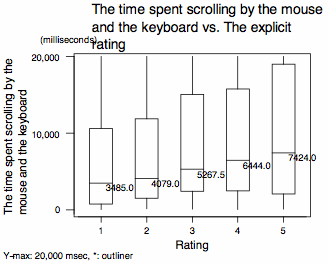
\includegraphics[width=7.5cm]{image/scroll.png}
  \caption{Time spent scrolling \citet{claypool2001}}
  \label{pic:scrolltime}
\end{figure}
\begin{figure}[h]
  \centering
  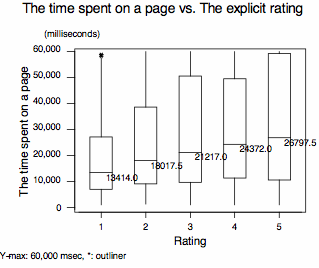
\includegraphics[width=7.5cm]{image/time.png}
  \caption{Time spent on a page \citet{claypool2001}}
  \label{pic:time}
\end{figure}

%\todo{explanations of the images}


In order to collect implicit user ratings by timing how long the website is in focus, the truncated mean time all users spend on the item page is used as a benchmark.
\begin{definition}[Truncated Mean]
  The truncated mean (tm) is calculated the same way as the average mean after discarding a specific percentage of the highest and lowest values.
  Let $n \in \mathbb{N}$, V be a set of sorted numbers and p be a percentage with $0 \leq p < 0.5$.
  Let $k = np$ be the trimmed value, $r = n - 2k$ be the remaining values, $v_j \in V$ and $j \in \mathbb{N}$.
  Then the following formula represents the truncated mean.
  \begin{displaymath}
    Truncated Mean = \sum_{j=k+1}^{n-k}{v_j} \cdot \frac{1}{r}
  \end{displaymath}
\end{definition}
The percentages of the two rating processes result out of the two diagrams of figure ~\ref{pic:scrolltime} and figure ~\ref{pic:time}.%todo more detail
The following paragraph explains the rating of the item page in relation to the truncated mean time.
\todo{Add diagrams, maybe write the itemization as a text}
\begin{itemize}
  \item If the user spends less than 10\% of the truncated mean time on the item page it is used as a rating of 1.
  \item If the user spends less than the truncated mean time minus 20\% on the webpage it is used as a rating of 2.
  \item If the user spends plus minus 20\% of the truncated mean time on the item page, it is used as a rating of 3.
  \item If the user spends longer than the truncated mean time plus 20\% on the webpage it is used as a rating of 4.
\end{itemize}
A rating of 5 can only be achieved if a user does a predefined user interaction on the web page.
The reason behind this choice is that users tend to make breaks while surfing the internet.
Thus, the user leaves the current browser window open but is not actively working on this website.
Therefore it is possible that a user is on a break and the currently active browser window might not be interesting for him in that moment.
Such a predefined user interaction can be used as an indicator that a user likes an item.
A possible predefined user interaction could be an up-vote or the writing of a comment or answer. 
A similar scale is chosen for determining the rating of a user by the time a user scrolls.
\begin{itemize}
  \item If the user scrolls less than 40\% of the truncated mean time on the item page it is used as a rating of 1.
  \item If the user scrolls between 40\% and 80\% of the truncated mean time on the webpage it is used as a rating of 2.
  \item If the user spends plus minus 20\% of the truncated mean time on the item page, it is used as a rating of 3.
  \item If the user spends between the truncated mean time plus 20\% and 60\% on the webpage it is used as a rating of 4.
  \item If the user scrolls longer than the truncated mean time plus 60\% it is used as a rating of 5
\end{itemize}
Due to the fact that scrolling is an active process and the user has to be in front of the computer a rating of 5 is achievable in this method.
First of all both implicit ratings - the time a user spends on a website and the time a user scrolls - are determined separately.
Afterwards the average of both ratings is calculated and used as the total rating.
%todo add weighting factor
\begin{displaymath}
  total rating = \frac{rating_{time} + rating_{scroll}}{2}
\end{displaymath}
%\todo{add this to evaluation}The concept is build upon measurements of a field experiment of 75 students by \citet{claypool2001}, though due to the lack of time it wasn't possible to test this concept on a large user base.
If a user returns to an item site the new rating is added onto the previous rating with a maximum sum of 5.
This rating calculation results from the observation that users tend to revisit websites they were interested in in the past and which might help them with their current research.
It was considered to generally rate all websites that were revisited with the highest rating of 5 but this concept was abandoned because a user might be revisiting a formally uninteresting website unintentionally. %\todo{find a source}

As mentioned above \citet{claypool2001} research group bases its results on a field experiment of over 80 people browsing over 2500 Web pages.
The total rating concept is strongly build upon these results.
It would have been desirable to conduct a field experiment for the concept of the total rating but unfortunately due to the lack of time it was not possible.
%\todo{eligable to conduct such a field experiment in the future} 
%describe the google news approach, explain the changes that where made and why.

%%source of definitions
%%why start with finite automata why create deterministic finite automata and how
\newpage
\section{Tagging}
In order to recommend items with a matching subject on a website, the newly developed system needs to be able to filter the items based on their content.
Therefore the keywords of the item content are used as tags in order to reflect the content of the items. %\todo{improve}
%The content can be described with the use of tags, these tags are the keywords of the content.
In the context of economics the \emph{ZBW} provides the \emph{STW Thesaurus for Economics}.
The \emph{STW Thesaurus for Economics} provides vocabulary on any economic subject and includes about 19000 terms and 6000 standardized keywords which can be used to match words from a text.\footnote{STW Thesaurus for Economics url: http://zbw.eu/stw/versions/latest/about}
It, thus, provides a good basis for the tagging process.
However, the \emph{STW Thesaurus for Economics} only includes the basic form of the words while excluding most of the words with affixation.
Due to this it is not sufficient to check whether the words from the items are equal to the words from the \emph{STW Thesaurus for Economics}.
So, the challenge for this tagging process is to find the correct words in the \emph{STW Thesaurus for Economics} even though the words from the item might not correspond directly to the words in the \emph{STW Thesaurus for Economics}.
One possible solution for such a task is to reduce each word from the text to its stem.\todo{definition stem}
Such a task is called stemming and is usually done by using predefined rules on the words. 
A rule is usually a combination of the minimum number of letters in a word, plus the suffix that should be changed and the replacement for the suffix.
More advanced algorithms might also use rules for prefix reduction and detecting irregular changes of the stem according to \emph{Caumanns A Fast and Simple Stemming Algorithm for German Words}.
For example a predefined rule might be '3+ies' $\rightarrow$ 'y'.
So, the word \emph{libraries} would be reduced to \emph{library}.
Thus it is important that the stemming algorithm has all necessary rules for each supported language.\\
Another challenge for using the stemming algorithm is that all words in the basis for the tagging process must be in the stem form. 
Otherwise the algorithm might reduce a word to its stem that would match in its original form.
Due to these maintenance problems it was decided that the stemming algorithm is not suitable for the developed system.
Another possible solution for the problem is to calculate the differences between the words from the text and the words from the basis for the tagging process.
This difference can be used as an indicator whether the words are similar or not.
If they are in a predefined difference range the words can be used as tags.%\todo{read this for a second time}
This creates the need for a metric that indicates the difference or distance between two words.
A practical metric for such a task is the \emph{levenshtein distance} which will be explained in the following section.
\subsection{Levenshtein Distance}

The \emph{levenshtein distance} calculates the minimum numbers of substitutions, insertions and deletions that are needed to change one word into another.
The following example explains the \emph{levenshtein distance} for the words \emph{library} and \emph{libraries}.
The algorithm has to perform two deletions and one substitution in order to create the word \emph{library} out of the word \emph{libraries}.
If it creates the word \emph{libraries} out of the word \emph{library} it has to perform a substitution and two insertions.
\begin{displaymath}
  {library \leftrightarrow librari \leftrightarrow librarie \leftrightarrow libraries}
\end{displaymath}
Both processes result in a \emph{levenshtein distance} of three.
So, the \emph{levenshtein distance} is zero if the words are equal and adds one to the result if it has to perform a substitution, an insertion or a deletion of a letter. 
For a more detailed description compare algorithm ~\ref{alg:levDist}.
% \todo{find better solution to move 'if'}
%   $levDist_{a,b}(i,j) = $
%   \begin{cases}
%     max(i,j) \quad \quad \quad \quad \quad \quad \quad \quad \quad \quad \quad \quad \quad \quad \text{if min(i,j) = 0} \\
%     min \begin{cases}
%         levDist_{a,b}(i-1, j)+1 \\
%         levDist_{a,b}(i, j-1)+1 & \text{else}\\
%         levDist_{a,b}(i-1, j-1) + [a_i \neq b_i] 
%       \end{cases}
%   \end{cases}\\
% This can be directly translated into a recursive algorithm. 
\begin{algorithm}
  \caption{Recursive Levenshtein Distance Algorithm}\label{alg:levDist}
  \begin{algorithmic}[1]
    \Procedure{LevenshteinDistance}{$s: String, t: String$}
    \State $lenS\gets length(s)$
    \If{lenS = 0}
      \State \textbf{return} $lenT$
    \EndIf
    \If{lenT = 0}
      \State \textbf{return} $lenS$
    \EndIf

    \If{s[lenS-1] = t[lenT-1]}\Comment{test if last characters of the strings match}
      \State $cost\gets 0$
    \Else
      \State $cost\gets 1$
    \EndIf

    \Comment{The first recursive call represents a deletion, the second represents an insertion and the third represents a substitution or a correct letter}
    \State \textbf{return} minimum of\par
    $LevenshteinDistance(s[0..lenS-1], t) +1,$\par 
    $LevenshteinDistance(s, t[0..lenT-1) +1,$\par 
      $LevenshteinDistance(s[0..lenS-1], t[0..lenT-1]) + cost)$ 

    \EndProcedure
  \end{algorithmic}
\end{algorithm}



The direct implementation of the \emph{levenshtein distance algorithm} has a complexity of O(mn) with m size of the first word and n size of the second word. 
Therefore it is a good utility to better understand the \emph{levenshtein distance} in general, but it is not feasible for a software that should work in production mode. 
\subsection{Optimized Levenshtein distance algorithm}
%definitions
The following definitions are based on the book \citet{automata2003}.
\begin{definition}[Non Deterministic Finite Automata]
  A non deterministic finite automata is a 5-tupel of the form $\mathcal{A} = (Q, \Sigma, q_0, \Delta, F)$. 
  \begin{itemize}
    \item Q is a finite set of the states
    \item $\Sigma$ is a finite set of input symbols
    \item $q_0 \in Q$ is the initial state
    \item $F \subset Q$ is a subset that contains the final states
    \item $\Delta$ is a relation of the form $\Delta \subset Q \times \Sigma \times Q$
  \end{itemize}
  $\mathcal{A}$ is called finite exactly when $Q$ is finite. Furthermore $\Sigma^*$ is the set of words over $\Sigma$ and $\epsilon$ is the empty word.
\end{definition}
\begin{definition}[Deterministic Finite Automata]
  $\mathcal{A}$ is deterministic if for all $p \in Q$ and all $a \in \Sigma$ exists exactly one state $q \in Q$ with $(p, a, q) \in \Delta$. In this case $\Delta$ is written as a function $\delta : Q \times \Sigma \rightarrow Q$.
\end{definition}
\begin{definition}[Path]
  A path for $\mathcal{A}$ is a series $\pi = p_0 a_1 p_1 a_2 \dots a_n p_n$, $(p_i, a_{i+1}, p_{i+1}) \in \Delta$ and $0 \leq i \leq n-1$. The length of $\pi$ is n and the label for $\beta(\pi)$ is $a_1 a_2 a_3 \dots a_n$.
\end{definition}
%\todo{$\beta$ explanation}
\begin{definition}[Path shortwriting]
  The function $\beta(\pi)$ maps a path $\pi$ to a label $\omega$.
  $\mathcal{A}: p \xrightarrow[]{\omega} q$ with $\omega \in \Sigma^*$ states, that a path $\pi$ for $\mathcal{A}$ from p to q with label $\beta(\pi) = \omega$ exists.
\end{definition}
\begin{definition}[Automata accepts a word]
  $\mathcal{A}$ accepts $\omega \in \Sigma^*$, if and only if $p \in I, q \in F$ exists with $\mathcal{A}$: $p \xrightarrow[]{\omega} q$. For $\mathcal{A}$ let $\mathcal{L}(\mathcal{A})=\{\omega \in \Sigma^*$ | $\mathcal{A}$ accepts $\omega\}$ be the language that $\mathcal{A}$ accepts.
\end{definition}

The following definitions are based on \citet{schulz2002}
\begin{definition}[Formal Levenshtein Distance]
  The levenshtein distance between two words $V, W \in \Sigma^*$ is the minimal number of edit operations (substitutions, deletions or insertions) that are needed to transform V into W.
  $d_L(V,W)$ denotes the levenshtein distance between V and W.
\end{definition}
\begin{definition}
  $\mathcal{L}_{Lev}(n, W)$, $n \in \mathbb{N}$ and $W \in \Sigma^*$ is the set that denotes all words $V \in \Sigma^*$ such that $d_L(W,V) \leq n$.
\end{definition}

\begin{definition}[Degree Levenshtein Automata]
  Let $W \in \Sigma^*$ and $n \in \mathbb{N}$. A finite state automaton A is a Levenshtein automaton of degree n for W if and only if $\mathcal{L}(A) = \mathcal{L}_{Lev}(n,W)$.
\end{definition}

An optimized version of the \emph{levenshtein distance algorithm} that uses a \emph{levenshtein automata} is described by \citet{Baeza-Yates96aunified}.
The purpose of the \emph{levenshtein automata} is to decide whether $d_L(W,V)$ is smaller than a specific $n \in \mathbb{N}$ with $V \in \Sigma^*$.
So, it is possible to decide if a word from a question is similar to a word from the \emph{STW Standard Thesaurus}, similar in the meaning it has a \emph{levenshtein distance} smaller than n.
Therefore $\Sigma$ contains the alphabet \{a,\ldots,z,A,\ldots,Z\}.
The states in Q of the \emph{levenshtein automata} denote the current position in the original word W, written as i and the current \emph{levenshtein distance} between $\omega$ and W, written as j, with $\omega$ prefix of V.
The label of such a state is $i^j$.
Thus the initial state $q_0 \in Q$ is $0^0$.
The final states $f \in F$ are all states where i equals |W| and j is smaller than n.\\
Let $\omega_{correct}$ be the correct letter after state $i^j$.
The relation $\Delta: (Q \times \Sigma \times Q)$ has the following elements.
\begin{itemize}
  \item $(i^j, \sigma, (i+1)^j)$ if $\sigma = \sigma_{correct}$ 
  \item $(i^j, \sigma, i^{(j+1)})$ if $\sigma$ is inserted after state $i^j$ and $(j+1) < n$
  \item $(i^j, \sigma, (i+1)^{(j+1)})$, if $\sigma$ is substituted by $\sigma_{correct}$ and $(j+1) < n$
  \item $(i^j, \sigma, (i+1)^{(j+1)})$, if $\omega_{correct}$ is deleted
\end{itemize}
The elements are not exclusive, therefore all of these cases can be possible after reading only one letter.
% \begin{math}
% (i^j, \sigma) \rightarrow \begin{cases}
%   (i+1)^j & \text{if correct}\\
%   (i)^{(j+1)} & \text{if insertion}\\
%   (i+1)^{(j+1)} & \text{if substitution or deletion}\\
%   empty & \text{if j is equal to n}
% \end{cases}
% \end{math}

\begin{figure}[h]
  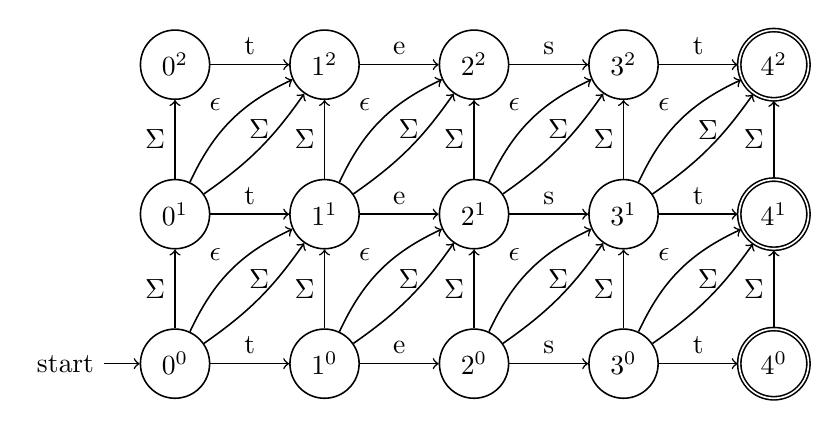
\begin{tikzpicture}[->,auto,line width=0.2mm] 
    %0,0 row
    \node[state] (q_2) {$0^2$}; 
    \node[state] (q_1) [below =of q_2] {$0^1$}; 
    \node[state,initial] (q_0) [below =of q_1] {$0^0$}; 

    %1,0 row t
    \node[state] (q_5) [right =of q_2] {$1^2$}; 
    \node[state] (q_4) [right =of q_1] {$1^1$}; 
    \node[state] (q_3) [right =of q_0] {$1^0$}; 

    %2,0 row e
    \node[state] (q_8) [right =of q_5] {$2^2$}; 
    \node[state] (q_7) [right =of q_4] {$2^1$}; 
    \node[state] (q_6) [right =of q_3] {$2^0$};

    %3,0 row s
    \node[state] (q_11) [right =of q_8] {$3^2$}; 
    \node[state] (q_10) [right =of q_7] {$3^1$}; 
    \node[state] (q_9) [right =of q_6] {$3^0$};

    %4,0 row t
    \node[state, accepting] (q_14) [right =of q_11] {$4^2$}; 
    \node[state, accepting] (q_13) [right =of q_10] {$4^1$}; 
    \node[state, accepting] (q_12) [right =of q_9] {$4^0$};

    %path deletion 0,0
    \path[->] 
    (q_0) edge node {$\Sigma$} (q_1)
    (q_1) edge node {$\Sigma$} (q_2);
    %path 0,0 -> 1,0
    \path[->] 
    %correct path
    (q_0) edge  node {t} (q_3)
    (q_1) edge  node  {t} (q_4)
    (q_2) edge  node  {t} (q_5)

    %insertion substitution
    (q_0) edge[bend right=10]  node[above,midway] {$\Sigma$} (q_4)
    (q_0) edge[bend left=20]  node  {$\epsilon$} (q_4)


    (q_1) edge[bend right=10]  node[above,midway] {$\Sigma$} (q_5)
    (q_1) edge[bend left=20]  node  {$\epsilon$} (q_5);

    %path deletion 1,0
    \path[->] 
    (q_3) edge node {$\Sigma$} (q_4)
    (q_4) edge node {$\Sigma$} (q_5);

    %path 1,0 -> 2,0
    \path[->] 
    %correct path
    (q_3) edge  node {e} (q_6)
    (q_4) edge  node  {e} (q_7)
    (q_5) edge  node  {e} (q_8)

    %insertion substitution
    (q_3) edge[bend right=10]  node[above,midway] {$\Sigma$} (q_7)
    (q_3) edge[bend left=20]  node  {$\epsilon$} (q_7)


    (q_4) edge[bend right=10]  node[above,midway] {$\Sigma$} (q_8)
    (q_4) edge[bend left=20]  node  {$\epsilon$} (q_8);


    %path deletion 2,0
    \path[->] 
    (q_6) edge node {$\Sigma$} (q_7)
    (q_7) edge node {$\Sigma$} (q_8);

    %path 1,0 -> 2,0
    \path[->] 
    %correct path
    (q_6) edge  node {s} (q_9)
    (q_7) edge  node  {s} (q_10)
    (q_8) edge  node  {s} (q_11)

    %insertion substitution
    (q_6) edge[bend right=10]  node[above,midway] {$\Sigma$} (q_10)
    (q_6) edge[bend left=20]  node  {$\epsilon$} (q_10)


    (q_7) edge[bend right=10]  node[above,midway] {$\Sigma$} (q_11)
    (q_7) edge[bend left=20]  node  {$\epsilon$} (q_11);

    %path deletion 3,0
    \path[->] 
    (q_9) edge node {$\Sigma$} (q_10)
    (q_10) edge node {$\Sigma$} (q_11);

    %path 3,0 -> 4,0
    \path[->] 
    %correct path
    (q_9) edge  node {t} (q_12)
    (q_10) edge  node  {t} (q_13)
    (q_11) edge  node  {t} (q_14)

    %insertion substitution
    (q_9) edge[bend right=10]  node[above,midway] {$\Sigma$} (q_13)
    (q_9) edge[bend left=20]  node  {$\epsilon$} (q_13)


    (q_10) edge[bend right=10]  node[above,midway] {$\Sigma$} (q_14)
    (q_10) edge[bend left=20]  node  {$\epsilon$} (q_14);

    %path deletion 3,0
    \path[->] 
    (q_12) edge node {$\Sigma$} (q_13)
    (q_13) edge node {$\Sigma$} (q_14);


  \end{tikzpicture}
  \caption{A non deterministic levenshtein automata for the word \emph{test} with degree 2}
  \label{ndla}
\end{figure}
The automata in example ~\ref{ndla} is a non deterministic levenshtein automata for the word \emph{test}.
In the following description the \emph{levenshtein automata} represents the word $W \in \Sigma^*$ and $\sigma \in \Sigma$ is the currently read letter.
$\Sigma$ indicates that any element from $\Sigma$ is accepted on this path.
The initial state $0^0$ is in the bottom left corner.
If $\sigma$ is a correct letter it follows the horizontal path in the automata.
A vertical path is an insertion of a letter $l \in \Sigma$ into the word W which is possible for any $\sigma$.
A diagonal path can be a deletion of a letter $l \in W$ with the empty word $\epsilon$ or a substitution of $\sigma$ for any $\sigma$.
Therefore after reading the letter 't' in the initial state $0^0$ the automata can be in five different states namely $0^1$, $1^2$, $1^1$, $2^2$ and $1^0$.
%\todo{explanation of the five different states}
Evaluating a non deterministic levenshtein automata is computational complex due to the fact that there can be a large number of active states at the same time. 
Thus it is necessary to convert a non deterministic automata to a deterministic automata before using it to find tags.
The process of generating a deterministic automata with a non deterministic automata is called \emph{powerset construction}.

\subsubsection{Powerset Construction}
The process of creating a \emph{deterministic levenshtein automata} out of an \emph{non deterministic levenshtein automata} is based on the \emph{powerset construction} from the book \emph{Introduction to Automata Theory, Languages, and Computation} by \citet{automata2003}.
Given a \emph{non deterministic levenshtein automata} the construction of an equivalent \emph{deterministic levenshtein automata} is described below. 
\begin{itemize}
  \item Create $q_0'$ as a set with original $q_0$ and all states that are reachable with an $\epsilon$ path.
  \item $Q' \subseteq 2^Q$, thus all $q \in Q'$ are subsets of Q.
  \item $\delta(R,a) = \{q \in Q$ | $\exists r \in R$ with (r, a, q) $\in \Delta$ or (r, $\epsilon$, p) and (p, a, q) $\in \Delta\}, R \subseteq Q$. %(r, a, p) and (p, $\epsilon$, q) $\in \Delta$ or 
  \item F' includes all $q \in Q'$ that include $f \in F$
\end{itemize}
Therefore the new \emph{deterministic levenshtein automata} is (Q', $\Sigma$, $q_0'$, $\delta$, F').


\newpage
Deterministic Levenshtein automata example for the word test with max \emph{levenshtein distance} 1.
%\todo{finish automata}
\begin{figure}[h]
  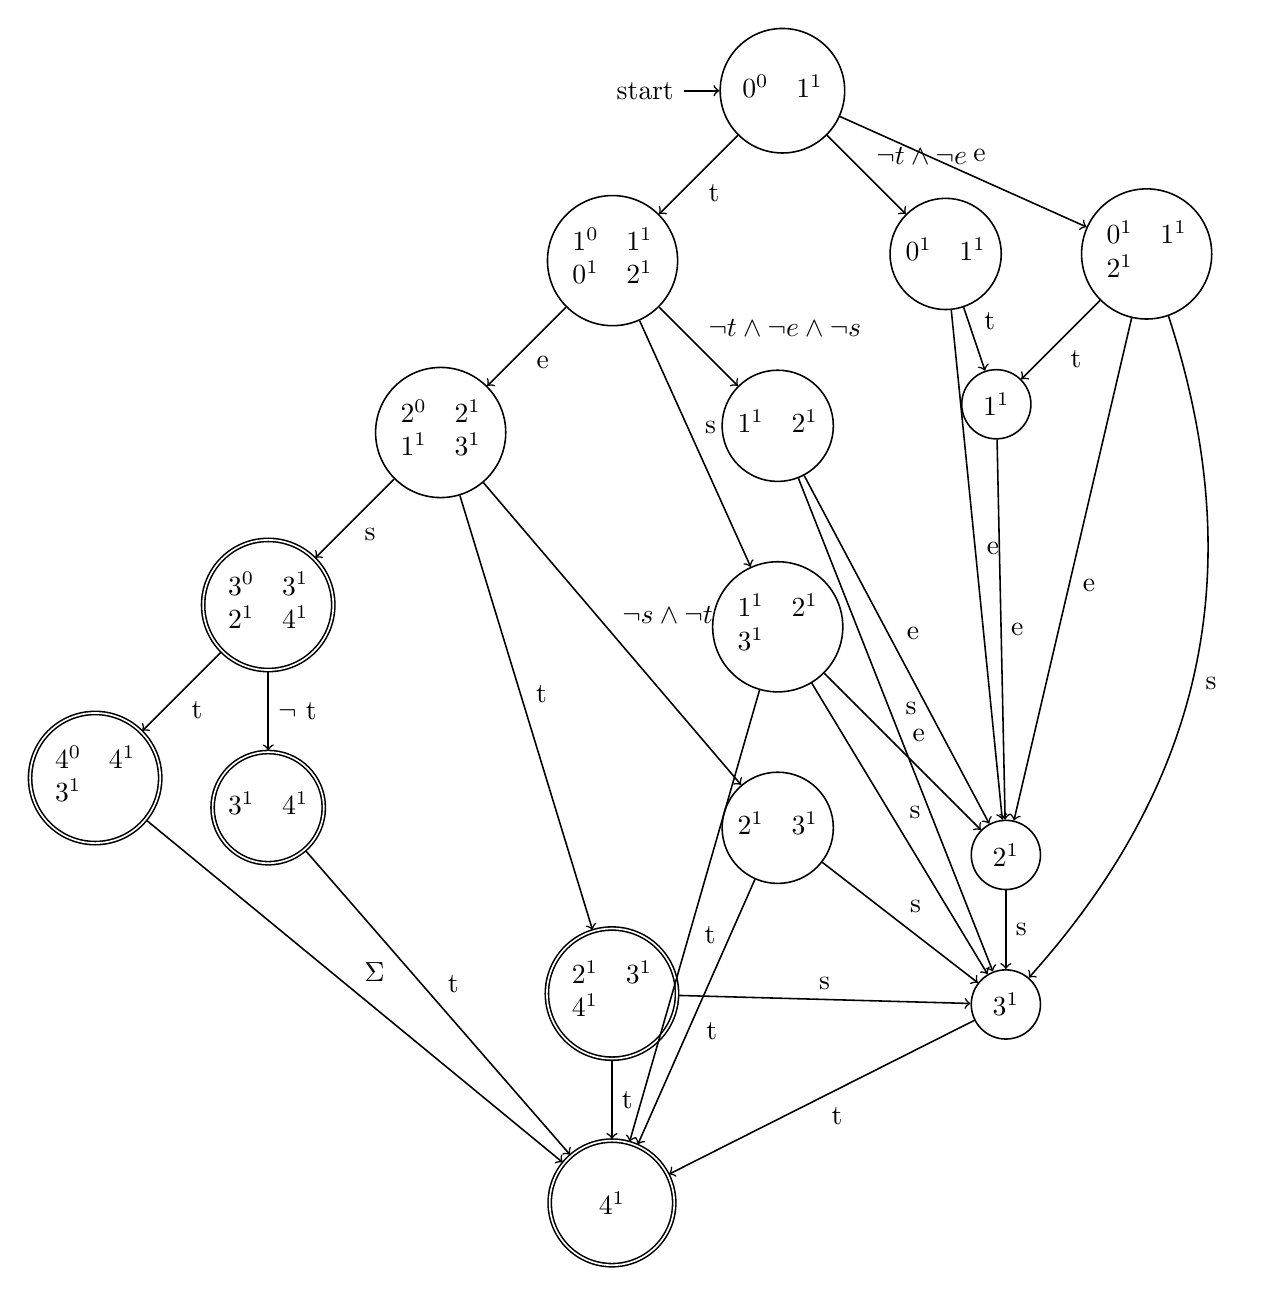
\begin{tikzpicture}[->,auto,line width=0.2mm] 
    \node[state,initial, minimum size=4.5em] (0_0-1_1) {$\begin{matrix} 0^0 & 1^1 \end{matrix}$}; 
    %correct path
     \node[state] (1_0-1_1-0_1-2_1) [below left=of 0_0-1_1] {$\begin{matrix} 1^0 & 1^1\\ 0^1 & 2^1 \end{matrix}$}; 
     \node[state] (2_0-2_1-1_1-3_1) [below left=of 1_0-1_1-0_1-2_1] {$\begin{matrix} 2^0 & 2^1\\ 1^1 & 3^1 \end{matrix}$}; 
     \node[state, accepting] (3_0-3_1-2_1-4_1) [below left=of 2_0-2_1-1_1-3_1] {$\begin{matrix} 3^0 & 3^1\\ 2^1 & 4^1 \end{matrix}$}; 

     \node[state, accepting] (4_0-4_1-3_1) [below left=of 3_0-3_1-2_1-4_1] {$\begin{matrix} 4^0 & 4^1\\ 3^1 \end{matrix}$}; 

     %first not t,e
     \node[state] (0_1-1_1) [below right=of 0_0-1_1] {$\begin{matrix} 0^1 & 1^1\end{matrix}$}; 

     %first e
     \node[state] (0_1-1_1-2_1) [right=of 0_1-1_1] {$\begin{matrix} 0^1 & 1^1\\ 2^1 \end{matrix}$}; 

      %q1 edges
     \node[state] (1_1-2_1) [below right=of 1_0-1_1-0_1-2_1] {$\begin{matrix} 1^1 & 2^1 \end{matrix}$}; 
     \node[state] (1_1-2_1-3_1) [below =of 1_1-2_1] {$\begin{matrix} 1^1 & 2^1 \\ 3^1 \end{matrix}$}; 

     %elementar
     \node[state] (1_1) [below left=of 0_1-1_1-2_1] {$1^1$}; 
     \node[state] (2_1) [below right=8em of 1_1-2_1-3_1] {$2^1$}; 
     \node[state] (3_1) [below =of 2_1] {$3^1$}; 



     \node[state, accepting] (3_1-4_1) [below =of 3_0-3_1-2_1-4_1] {$\begin{matrix} 3^1 & 4^1 \end{matrix}$}; 

     \node[state] (2_1-3_1) [below =of 1_1-2_1-3_1] {$\begin{matrix} 2^1 & 3^1 \end{matrix}$}; 
     \node[state, accepting] (2_1-3_1-4_1) [below left=of 2_1-3_1] {$\begin{matrix} 2^1 & 3^1\\ 4^1 \end{matrix}$}; 
     \node[state, accepting, minimum size=4.5em] (4_1) [below =of 2_1-3_1-4_1] {$4^1$}; 
     \path[->]
     (0_0-1_1) edge node {$\neg t \wedge \neg e$} (0_1-1_1)
     (2_0-2_1-1_1-3_1) edge node {$\neg s \land \neg t$} (2_1-3_1)
     (2_0-2_1-1_1-3_1) edge node {t} (2_1-3_1-4_1)
     (0_0-1_1) edge node {e} (0_1-1_1-2_1)
     (1_0-1_1-0_1-2_1) edge node {$\neg t \wedge \neg e \wedge \neg s$} (1_1-2_1)
     (1_0-1_1-0_1-2_1) edge node {s} (1_1-2_1-3_1)
     (0_1-1_1) edge  node {t} (1_1)
     (0_1-1_1) edge  node {e} (2_1)
     (1_1) edge  node {e} (2_1)
     (2_1) edge  node {s} (3_1)
     (3_1) edge  node {t} (4_1)
     (1_1-2_1) edge  node {e} (2_1)
     (1_1-2_1) edge  node {s} (3_1)
     (3_0-3_1-2_1-4_1) edge node {$\neg$ t} (3_1-4_1)
     (3_1-4_1) edge node {t} (4_1)
     (0_0-1_1) edge  node {t} (1_0-1_1-0_1-2_1)
     (1_0-1_1-0_1-2_1) edge  node  {e} (2_0-2_1-1_1-3_1)
     (2_0-2_1-1_1-3_1) edge  node  {s} (3_0-3_1-2_1-4_1)
     (3_0-3_1-2_1-4_1) edge  node  {t} (4_0-4_1-3_1)
     (2_1-3_1-4_1) edge  node {t} (4_1)
     (2_1-3_1-4_1) edge  node {s} (3_1)
     (2_1-3_1) edge  node {s} (3_1)
     (2_1-3_1) edge  node {t} (4_1)
     (0_1-1_1-2_1) edge  node {t} (1_1)
     (0_1-1_1-2_1) edge  node {e} (2_1)
     (0_1-1_1-2_1) edge[bend left=30]  node {s} (3_1)
     (1_1-2_1-3_1) edge  node {e} (2_1)
     (1_1-2_1-3_1) edge  node {s} (3_1)
     (1_1-2_1-3_1) edge  node {t} (4_1)
     (4_0-4_1-3_1) edge  node  {$\Sigma$} (4_1);


  \end{tikzpicture}
  \caption{A deterministic levenshtein automata for the word \emph{test} with degree 1}
  \label{dla}

\end{figure}


% \begin{itemize}
%   \item $\Sigma$ is the complete alphabet
%   \item Each state in Q denotes for an insert word $\omega \in \Sigma^*$ the number of matching letters together with $d_L(\omega,W)$
%   \item The initial state $q_0$ is the state with insert count 0 and \emph{levenshtein distance} 0
%   \item The function $\delta$ is the known function $\delta : Q \times \Sigma \rightarrow Q$. \todo{definiere delta}
%   \item The set of final states F contains all states where the correct letter count is equal to the size of the original word W.
% \end{itemize}

Let $(Q, \Sigma, q_0, \Delta, F)$ be a \emph{non deterministic levenshtein automata} for the word \emph{test} with maximum \emph{levenshtein distance} 1 \footnote{This is the automata from figure ~\ref{ndla} without the first row}. 
Then the \emph{deterministic levenshtein automata} $DLA = (Q', \Sigma, q_0', \delta, F')$ from figure ~\ref{dla} is the output from the powerset construction.
Consequently the DLA can only have one active state at a time and accepts all words V from $\Sigma^*$ with $d_L('test', V) \leq 1$. 
This deterministic finite automata with degree $n \in \mathbb{N}$ for a word $W \in \Sigma^*$ can decide in linear time if a word $V \in \Sigma^*$ has $d_L(W,V) \leq n$. %\todo{source Lemma3}.

\begin{algorithm}
  \caption{Levenshtein Automata is in distance}\label{alg:levDistIsInDist}
  \begin{algorithmic}[1]
    \Procedure{isInDistance}{$automata: DeterministicFiniteAutomata, term: String$}
    \State $i\gets 0$
    \State $currentStates\gets (0,0)$\Comment{add the initial state}
    \While{currentStates.size > 0 AND i < term.length}
      \State $c\gets term[i].toLowerCase$\Comment{c gets the current active lower cased letter}
      \State $currentStates\gets automate.nextState(currentStates, c)$
      \State $i\gets i+1$
    \EndWhile
    \If{currentStates includes a final state}
      \State \textbf{return} true
    \Else
      \State \textbf{return} false
    \EndIf

    \EndProcedure
  \end{algorithmic}
\end{algorithm}

The maximum distance for a given word $W \in \Sigma^*$ depends on the length n of W.
%\todo{try to find the nouns of the content cause these are the keywords of the text}
%todo the word W is the plural form therefore it should be if n > 7 degree 3 is used otherwise 1
A word with length of $n\leq3$ in the \emph{Standard Thesaurus Economics} is usually an abbreviation and therefore is only used as a direct match.
A word with length of $n>3$ is used with a maximum distance of three due to the reason that most of the plural forms involve three changes (substitution, insertion and deletion) in the German language.%\todo{add source Die Pluralbildung im Deutschen: Eine Untersuchung an Hand der Optimalit�tstheorie: "German Noun Plural reconsidered" von Dieter Wunderlich explain that there are 15 different plural forms \dots}

%optimization generate dfa directly or use table based evaluation method

%Lemma 6 For any fixed number n, given two words W and V of length w and v respectively, it is decidable in time O(max(w, v)) if the Levenshtein distance between W and V is <= n.

%\todo{add more explanation how the levenshtein automata is integrated into the system}
To get back to the original problem this paragraph explains the application of the \emph{levenshtein distance automata} to find the right tags for a text.
The overall tagging concept is to calculate for every word from the text an automata and read all words from the \emph{STW Thesaurus for Economics} into each automata.
If a word from the \emph{STW Thesaurus for Economics} ends in a final state it is used as a tag for the text. 
A possible optimization would be to calculate once all the automata's for the complete \emph{STW Thesaurus for Economics} and to store it with an efficient data structure in a database.
Currently the \emph{STW Thesaurus for Economics} is stored in a triple store because it can easily be updated with the standard files from the website.
\todo{triple store definition}

\newpage
%why did I choose item-based and svd-based recommendations? why the combination of both
%description of item based recommendation, how do I use item based recommendations
%description of collaborative filtering, description of svd, how do I use this sort of recommendations
\section{Recommendation}
A recommendation system is a system that creates personalized item recommendations based on information about the items or the relationships between items and users.
These recommendations can be created by different types of recommendation systems that exploit different information about the users or items.
\subsection{Different types of recommendation systems}
%\todo{Describe different informations that are needed.}
The book \emph{Recommender Systems An Introduction} by \citet{recommender2011} distinguishes between the following four different kind of recommendation systems.
%These recommendation systems that are described below exploit either the relationship between the users 
\subsubsection{Collaborative recommendation}
Collaborative recommendations are recommendations based on similar interests of users.
So, if user A and user B are interested in similar items and user A shows interest in item I that is unknown to user B, than item I might be interesting for user B as well.
Due to the fact that this technique filters all items based on implicit collaboration of the users it is also known as \emph{collaborative filtering}.
For using the collaborative filtering approach no other information are needed than the relationship between users and items. 
Depending on the number of items in the system and the activity of the users of the system the process of collecting information about the relationship between the users and the items they are interested in might be needing some time.
Although it needs to collect initial data it is a good approach if the items that need to be recommended are unknown or additional information for the items would be hard to maintain.%\todo{read a second time more explanations needed?}
\subsubsection{Content-based recommendation}
In content-based recommendations the items are usually documents that should be recommended based on the content.
Thus, the content of the document is described by tags.
These tags can have an indicator that expresses the importance of the tag.
Therefore the documents can be filtered by the tags of the documents and ranked by the importance of the tags.
These tags can be maintained explicitly by the users of the systems or by tagging algorithms.
One advantage of content-based recommendation systems is that they do not require a large user base to achieve good recommendations for users.
A second advantage is that new items can be recommended to users immediately after the content has a description.
If the content is user generated the recommendation system can only recommend documents that fit the current context.
It has no information whether a user likes the content or not which can lead to poor recommendations.
All in all, content-based systems are a good choice if the system has to provide recommendations for quality documents.
As long as the documents have a description for the system.

\subsubsection{Knowledge-based recommendation}
The basic idea behind knowledge-based recommendation system is a system that has enough information about the items and the needs of the user and as such can recommend items based on matching the needs of the user and the features of the items.
Moreover the system has to use individual user requirements in order to create personalized recommendations. 
For example if a user would like to buy a new jacket for a summer camping trip in England the knowledge based system has to use the specific context in order to recommend a thin light rain jacket with the right size and price for the user.
These information are usually manually provided by the user and the maintainer of the system.
Furthermore not only the system needs to correctly interpret the information but the user needs to have the domain knowledge in order to provide the system with the correct information.
So, knowledge-based recommendation is a good approach if the system has to recommend items that are not frequently requested and no user history is available.
It is especially suited for applications in which items are not frequently bought such as expensive digital goods or cars. 

\subsubsection{Hybrid approaches}
All recommendation system approaches have advantages and disadvantages, therefore a combinations of the different approaches which are mentioned above could improve the user recommendations as long as the system has enough information about the items or users.

\subsubsection{Conclusion}
%\todo{improve this}
%not enough information for knowledge based system
%use tags to filter collaborative recommendations
%fall back for cold start problem
%new user / not logged in
%use top rated items for the subject
%if no items 
%use top rated items
Knowledge based systems require too much domain knowledge that is not accessible for user generated questions and answers, therefore knowledge based systems are not feasible for the system.
Collaborative recommendation systems have the \emph{cold start problem}, so they need an initial amount of user item relationship data in order to present good recommendations. 
Additionally, they have no information about the subject of the items and this might lead to a situation were a collaborative filtering system might recommend unapropriate items to the current context. 
Nonetheless collaborative filtering is the only approach that takes the interest of similar users into account. 
As such it is the only technique that is able to recommend items that are approved by similar users. 
Moreover the content-based systems have the disadvantage that they do not make use of the information whether or not a user likes a document.
Yet, they do not need to collect additional relationship information in order to recommend items.
For these reasons the described recommendation system uses a collaborative filtering technique with pre filtered content based on the tags for each item.

%%definitions Users, items, ratings, predictions
\subsection{Collaborative recommendation system}
As mentioned above a collaborative recommendation system recommends items to users based on the interest of similar users.
% -different collaborative recommendation techniques
% -user based nearest neighbor recommendations
% --Memory based approach best similarity measure pearson correlation 
% -item based
% --recommends items based on similar items
% -matrix factorization techniques
% --uses matrix factorization techniques to get latent data that is hidden in the user item matrix this data is used to create recommendations
% -probabilistic recommendation
% --Uses techniques from the probabilistic theory one of the main approaches of these techniques are to create groups of similar users, at runtime the probability for a user is calculated in which group he belongs and whether the group likes an item or not. Performance depends on the number of groups and the group size
The following definitions are based on \citet{recommender2011}
\begin{definition}[User]
  $U = \{u_1, u_2, u_3, \dots, u_n\}$ is a set with $u_i$ users from the recommendation system. With $n, i \in \mathbb{N}$ and $i \leq n$.
\end{definition}

\begin{definition}[Item]
  $I = \{i_1, i_2, i_3, \dots, i_n\}$ is a set with $i_j$ items from the recommendation system. With $n, j \in \mathbb{N}$ and $j \leq n$.
\end{definition}

\begin{definition}[Rating]
  R is an $n \times m$ matrix with $n = |I|$ and $m = |U|$. 
  Furthermore is $r_{n,m}$ a rating for item $n \in I$ and user $m \in U$ with $r_{n,m}$ entry in R and $r_{n,m} \in \{1, 2, 3, 4, 5\}$.
  If a user $k \in U$ has not rated an item $l \in I$ the entry $r_{l, k}$ remains empty.
  $\hat{I_u}$ is a set with all items $i \in I$ where $r_{i, u}$ is empty, $\tilde{I_u}$ is a set with all items i and $r_{i, u}$ is not empty.
\end{definition}

\begin{definition}[Prediction]
  A prediction is a rating $r_{i,u}$ for item $i \in I$ and user $u \in U$ with $r_{i,v}$ empty entry in $R$.
\end{definition}

\begin{definition}[Recommendation]
  Let $n \in \mathbb{N}$ and $u \in U$.
  A recommendation is a set of n predictions for a user u ordered by the values of the predictions.
\end{definition}

%There are different types of collaborative recommendation techniques.
%\todo{explain probabilistic and slope one and why you didn't choose them}

\subsubsection{Item-Based Recommendation}
The concept of item-based recommendation was introduced by \citet{sarwar2001}.
The idea behind this concept is that recommendations can be calculated based on similar items of the items that a user likes.
If $i, \in \hat{I_u}$ and $u \in U$, then the prediction for i can be calculated with the similarity between i and all items $j \in \tilde{I_u}$.
There are different possible ways to calculate the similarity between two items.
However, the similarity calculation with the best performance is \emph{adjusted cosine similarity} which is an optimized form of the \emph{cosine similarity}\footnote{see \citet{sarwar2001}}
\begin{definition}[Cosine Similarity]
  With i, j $\in \mathbb{N}^n$, n $\in \mathbb{N}$.
  \begin{equation}
    cos(\overrightarrow{i}, \overrightarrow{j}) = \frac{\overrightarrow{i} \cdot \overrightarrow{j}}{||\overrightarrow{i}||_2 \cdot ||\overrightarrow{i}||_2}
  \end{equation}
\end{definition}
If $\overrightarrow{i}, \overrightarrow{j}$ are rating vectors, the individual rating behaviour of a user needs to be taken into account to get better predictions with the similarities of $\overrightarrow{i}$ and $\overrightarrow{j}$.
Due to the fact that different users have different average ratings.
This results in the \emph{adjusted cosine similarity}.
\begin{definition}[Adjusted Cosine Similarity]
  Let $i,j \in Items$ and $\overline{r_u}$ be the average rating from user u.
  The cosine similarity can be transformed to the adjusted cosine similarity by subtracting the average user rating from the current rating.
  \begin{equation}
    sim(i, j) = \frac{\sum_{u \in U}{(r_{u, i} - \overline{r_u})(r_{u, j} - \overline{r_u})}}{\sqrt{\sum_{u \in U}(r_{u,i} - \overline{r_u})^2} \sqrt{\sum_{u \in U}(r_{u,j} - \overline{r_u})^2}}
  \end{equation}
\end{definition}
Researches show that the \emph{adjusted cosine similarity} has the best performance with attention to prediction accuracy compared to all other similarity measures for item based algorithms. [\citet{sarwar2001}]
The results of the cosine similarity are between -1 and 1 with 1 meaning identical, 0 meaning indifferent and -1 meaning opposite [\citet{wikiCosineSimilarity}].
Although the results vary between -1 and 1 those items that have a \emph{cosine similarity} of $\leq 0$ are too different and thus are not used for further calculations.
The user item predictions can be generated with the similarities by using the following formula.
\begin{definition}[Item Based Prediction]
  \begin{equation}
    pred(u, p) = \frac{\sum_{i \in \tilde{I_u}}{sim(i, p) \cdot r_{u, i}}}{\sum_{i \in \tilde{I_u}}{ sim(i, p)}}
  \end{equation}
\end{definition}
The item similarity calculations can be calculated offline on a regular basis - every day or weekly - depending on the activeness of the users and the amount of item changes.
So, the item based technique is a good choice for websites that need fast scalable recommendations because only the item predictions are calculated on time.
Furthermore the team of \emph{Sarwar et al} found out that the system only needs a subset of all items.
According to \emph{Sarwar et al} a sample of the 25 most similar items is needed to generate good recommendations [\citet{sarwar2001}].
Thus the on time calculation needs to find the top 25 most similar users in the similarity table and has to calculate the recommendations with these users instead of using all similar users.
Moreover, it is a tested concept for instance amazon.com uses item based recommendations for their product recommendations [\citet{amazon2003}]. 
To get back to the overall concept, the item based predictions are used in order to decrease the rating sparsity of the user-item table. 
So, more information about the user interest is available before the actual recommendations can be calculated.
In real world recommendation systems the user item ratings tend to be very sparse because most users only rate few items [\citet{recommender2011}].

\subsubsection{Example for Item-Based Recommendations}
The table in figure ~\ref{itemBasedTable} represents a user item relationship.\\

\begin{figure}[h]
  \centering
  \begin{tabular}{c c c c c c}
   &Item1 & Item2 & Item3 & Item4 & Item5 \\ 
  User1 & 5 & 3 & 4 & 4 & ?\\  
  User2 & 3 & 1 & 2 & 3 & 3\\ 
  User3 & 4 & 3 & 4 & 3 & 5\\ 
  User4 & 3 & 3 & 1 & 5 & 4\\ 
  User5 & 1 & 5 & 5 & 2 & 1\\ 
  \end{tabular}
  \caption{User Item Relationship Table}
  \label{itemBasedTable}
\end{figure}

  This example calculates the item based prediction for User1 and Item5
  \begin{displaymath}
   sim(Item5,Item1) = {{3\cdot3 + 5\cdot4 + 4\cdot3 + 1\cdot1} \over {\sqrt{3^2 + 5^2 + 4^2 + 1^2} \cdot \sqrt{3^2 + 4^2 + 3^2 + 1^2}}} = 0.99
  \end{displaymath}
  sim(Item5, Item1) = 0.99\\
  sim(Item5, Item2) = 0.74\\
  sim(Item5, Item3) = 0.72\\
  sim(Item5, Item4) = 0.94\\
  With these similarities the following prediction can be calculated.
  \begin{displaymath}
    pred(User1, Item5) = {{0.99 \cdot 5 + 0.74 \cdot 3 + 0.72 \cdot 4 + 0.94 \cdot 4} \over {0.99 + 0.74 + 0.72 + 0.94}} = 4.07
  \end{displaymath}

  As a result User1 would most likely rate Item5 with 4.07.

\subsubsection{Singular Value Decomposition}
The singular value decomposition is a matrix factorization technique that can be used to find latent factors in the rating patterns.
With these factors it is possible to find similar users and items.
The singular value decomposition was found in the late 1800 to early 1900 [\citet{historyOfSVD}].
Besides one of the main areas of application of the singular value decomposition today is information retrieval.
The basic idea behind the singular value decomposition based information retrieval is to match user queries to documents.
This is done by decomposing a term by document matrix and using the item vectors of the decomposition to find documents based on queries that are decomposed into term vectors [\citet{deerwester1990}].
\begin{definition}[Vector]
\end{definition}
\begin{definition}[Matrix]
\end{definition}
\begin{definition}[Linear Dependent, Linear Independent]
\end{definition}
\begin{definition}[Rank of a Matrix]
\end{definition}
\begin{definition}[Matrix Multiplication]
\end{definition}
\begin{definition}[Orthogonal Matrix]
\end{definition}
\begin{definition}[Eigenvalue of a Matrix]
\end{definition}

The singular value decomposition of an $m \times n$ matrix with rank r is a factorization of the form:
\begin{equation}
  SVD(M) = U \Sigma V^t
\end{equation}
U and V are orthogonal matrices with dimension $m \times r$ and $r \times n$. 
Furthermore $\Sigma$ is a rectangular diagonal matrix with dimension $r \times r$.
The diagonal values $\sigma_{i,i} \in \Sigma$ with $i \in \mathbb{N}$ have by convention the property $\sigma_{i,i} \geq \sigma_{i+1,i+1} > 0$.
The $\sigma_{i,i}$ are the none negative square roots of the eigenvalues of $AA^t$ and $A^tA$ \footnote{Due to the fact that $AA^t$ and $A^tA$ share the same eigenvalues.} [\citet{numericalLinearAlgebra}]. 
The columns of U are the corresponding eigenvectors to the eigenvalues of $AA^t$.
On the other hand are the columns of the Matrix V the corresponding eigenvectors to the eigenvalues of $A^tA$ \footnote{The eigenvalues are the squares of $\sigma_{i,i}$} [\citet{numericalLinearAlgebra}].
So, $AA^t \cdot u_i = \sigma_{i,i}^2 * u_i$.\\ %\todo{is this a reason why this spans the columns of the original matrix A?}
%\todo{U spans column space V spans row space}\\
To sum this up, the matrix U corresponds to the columns of the matrix A and the matrix V corresponds to the rows of the matrix A.
It is possible to obtain an optimal rank k approximation from matrix A, with $k \leq r$.
By setting all $\sigma_{i,i}$ with $i > k$ to zero [\citet{matrixAlgorithms}].
Thus $A_k = U_k \times \Sigma_k \times V_k^t$ yields the optimal rank k approximation.
As a result all column vectors $u_i$, with $i > k$, of matrix U will be multiplied by a zero vector from matrix $\Sigma_k$.
Due to the fact that matrix U represents the columns of matrix A and that the last rows of matrix U will be removed in order to generate the optimal rank k approximation of matrix A, it is possible to generate a good approximation of the user interests by removing the last rows of matrix U.\footnote{A user from the system is represented by a column in the matrix A}
The two dimensional matrix $U_2$ is created by removing all rows of matrix U up to the first two rows.
This matrix $U_2$ can be seen as a value table that can be represented by a graph.
Therefore, it enables a graphical presentation of the user similarities.
Furthermore the user similarities can be calculated by using the cosine similarity between the columns of $U_k$.\\
After calculating the similarities for each user, the recommendations for $user_a \in U$ are calculated.
For this task the algorithm takes all similar users $U_{sim}$ for $user_a$.\\
Afterwards it uses the top rated items from all $user_b \in U_{sim}$ that are not rated by $user_a$ $I'_{user_a, user_b}$.
$\overline{r_a}$ denotes the average rating of user a.
Finally for each item $i \in I'_{user_a, user_B}$ the prediction is calculated.

\begin{displaymath}
  pred_{a, i} = \overline{r_a} + \frac{\sum_{b \in U_{sim}}{(r_{i, b} - \overline{r_b}) * similarity_{a, b}}}{\sum_{b \in U_{sim}}{similarity_{a, b}}}
\end{displaymath}

% def getCalculateUserPredictions(userId: Int, path: Array[String]): Future[HttpResponse] = {
%   val predictions = collection.mutable.HashMap[Int, List[(Int, Int, Double)]]()
%   for(s <- SimilarUsers.byUserId(userId, 5)){
%     val (similarUserId, similarity) = s.similarityByUserId(userId).get
%     if(similarity > 0) { 
%       for(rating <- Ratings.getUnknownItemsForUserByUser(userId, similarUserId))
%       {
%         predictions += rating.itemId -> addToList(predictions.get(rating.itemId), (similarUserId, rating.rating, similarity))
%       }
%     }
%   }
%   val predictionMap = predictions.flatMap((i: (Int, List[(Int, Int, Double)])) => Map(i._1.toString->calculatePrediction(userId, i._2).toString))
%   Future.value(createHttpResponse(Json.toJson(predictionMap)))
% }

% def calculatePrediction(userAId: Int, topItems: List[(Int, Int, Double)]): Double = {
%   if(topItems.length > 1){
%     val averageRatingA = Users.get(userAId).get.averageRating
%     val numerator = topItems.map{case(userBId: Int, rating: Int, similarity: Double) => {
%       val averageRatingB = Users.get(userBId).get.averageRating
%       (rating-averageRatingB)*similarity
%     }}.sum
%     val denominator = topItems.map(_._3).sum
%     val rating = averageRatingA + numerator/denominator
%     if(rating > 0) rating else 0
%   }
%   else 0
% }

%\todo{how to calculate predictions with these tables}
\newpage
Example for a singular value based recommendation\\
\begin{displaymath}
  \begin{tabular}{c c c c c c}
     &Item1 & Item2 & Item3 & Item4 & Item5 \\ 
     User1 & 5 & 3 & 4 & 4 &  \\  
    User2 & 3 & 1 & 2 & 3 & 3\\ 
    User3 & 4 & 3 & 4 & 3 & 5\\ 
    User4 & 3 & 3 & 1 & 5 & 4\\ 
    User5 & 1 & 5 & 5 & 2 & 1\\ 
  \end{tabular} 
\end{displaymath}

The following example calculates the rating prediction for \emph{User1} and \emph{Item5}.
A singular value decomposition for a user item relationship table is created in figure ~\ref{svdexample}.
The first two rows of matrix U are used to create a value table for a graph that represents the user similarities this is displayed in figure ~\ref{svdgraph}.
The \emph{cosine similarity} is used to calculate the following similarities.
\begin{displaymath}
  %User5: 0.402286&0.716108
  %User4: 0.455479&-0.486113
  %User3: 0.535742&-0.210593
  %User2: 0.342950&-0.316949
  %User1: 0.475467&0.325691
   sim(User1,User2) = {{0.475467\cdot0.342950 + 0.325691\cdot-0.316949} \over {\sqrt{0.475467^2 + 0.325691^2} \cdot \sqrt{0.342950^2 + (-0.316949)^2}}} = 0.222322
\end{displaymath}
\begin{itemize}
  \item sim(User1, User2) = 0.222322
  \item sim(User1, User3) = 0.561072
  \item sim(User1, User4) = 0.151704
  \item sim(User1, User5) = 0.896770
\end{itemize}
The following itemization contains the average user ratings.
\begin{itemize}
  \item $\overline{r_{User2}} = 2.4$
  \item $\overline{r_{User3}} = 3.8$
  \item $\overline{r_{User4}} = 3.2$
  \item $\overline{r_{User5}} = 2.8$
\end{itemize}
  With these similarities and average ratings the following prediction can be calculated.
  $pred(User1, Item5) =$\\ $4 + \frac{(3 - 2.4) \cdot 0.222322 + (5 - 3.8) \cdot 0.561072 + (4 - 3.2) \cdot 0.151704 + (1 - 2.8) \cdot 0.896770}{0.222322 + 0.561072 + 0.151704 + 0.896770} = 3.6254$\\
  As a result User1 would most likely rate Item5 with 3.6254.
  %todo This example underlines the need of removing the sparsity of a rating table because every empty entry \dots
\begin{figure}[h]
\begin{math}
  \begin{tabular}{c c c c c c}
     &Item1 & Item2 & Item3 & Item4 & Item5 \\ 
     User1 & 5 & 3 & 4 & 4 &  \\  
    User2 & 3 & 1 & 2 & 3 & 3\\ 
    User3 & 4 & 3 & 4 & 3 & 5\\ 
    User4 & 3 & 3 & 1 & 5 & 4\\ 
    User5 & 1 & 5 & 5 & 2 & 1\\ 
  \end{tabular} = 

  \begin{pmatrix}
    0.475467&0.325691&0.798636&-0.053513&-0.164835\\0.342950&-0.316949&0.082532&-0.250224&0.844099\\0.535742&-0.210593&-0.362530&-0.589189&-0.435955\\0.455479&-0.486113&-0.054206&0.729352&-0.146077\\0.402286&0.716108&-0.470107&0.235423&0.221199
  \end{pmatrix} \cdot \\
  \begin{pmatrix}
    15.627834&0.0&0.0&0.0&0.0\\0.0&5.104899&0.0&0.0&0.0\\0.0&0.0&3.541202&0.0&0.0\\0.0&0.0&0.0&2.426008&0.0\\0.0&0.0&0.0&0.0&0.534013
  \end{pmatrix} \cdot \\
  \begin{pmatrix} 
    0.46825&0.432206&0.46056&0.487586&0.379564\\-0.177671&0.42127&0.572180&-0.250389&-0.633148\\0.609379&-0.316926&-0.139853&0.322858&-0.635938\\-0.392214&0.489216&-0.480126&0.571026&-0.224148\\-0.473276&-0.544015&0.458702&0.518898&-0.019831
  \end{pmatrix}
\end{math}
\caption{Singular Value Decomposition of the User Item Relationship Table}
\label{svdexample}
\end{figure}

\begin{figure}
\begin{minipage}{0.3\textwidth}
\begin{math}
    \begin{pmatrix}
    0.475467&0.325691  \\ 0.342950&-0.316949  \\ 0.535742&-0.210593 \\ 0.455479&-0.486113  \\ 0.402286&0.716108 
  \end{pmatrix} 
\end{math}
\end{minipage}
\begin{minipage}{0.7\textwidth}
\begin{tikzpicture}[scale=3.0]
 \begin{scope}[thin,black,dot/.style={fill=blue,circle,inner sep=0pt,minimum size=3pt}]
   %x-y-Koordinatensystem
%  \draw[-latex] (90:-1) --++(90:2) node[left]{$y$};
%  \draw[-latex] (0:-1) --++(0:2) node[below]{$x$};
   \coordinate (x1) at (0, 0);
   \coordinate (x2) at (1, 0);
   \coordinate (y1) at (0, -1);
   \coordinate (y2) at (0, 1);
   \draw (x1) -- (x2) node[right]{$x$};
   \draw (y1) -- (y2) node[above]{$y$};
   \node [left] at (0,0) {$0.0$};
   \node [left] at (0,-1) {$-1.0$};
   \node [left] at (0,1) {$1.0$};
   \node [below] at (1,0) {$1.0$};


   \coordinate (user1) at (0.475467, 0.325691); 
   \node[dot] at (user1);
   \node [anchor=west] at (user1) {$User1$};

   \coordinate (user2) at (0.342950, -0.316949); 
   \node[dot] at (user2);
   \node [anchor=west] at (user2) {$User2$};

   \coordinate (user3) at (0.535742, -0.210593); 
   \node[dot] at (user3);
   \node [anchor=south west] at (user3) {$User3$};

   \coordinate (user4) at (0.455479, -0.486113); 
   \node[dot] at (user4);
   \node [anchor=west] at (user4) {$User4$};

   \coordinate (user5) at (0.402286, 0.716108); 
   \node[dot] at (user5);
   \node [anchor=west] at (user5) {$User5$};

   

   
 \end{scope}
\end{tikzpicture}
\caption{Similar Users based on Singular Value Decomposition}
\label{svdgraph}
\end{minipage}
\end{figure}

\subsection{The recommendation process}
The sparsity of the user item table is decreased by using item based predictions for user-item pairs that are not rated.
For this process the system uses the similarities between rated and not rated user-item pairs.
Therefore for each user (u) the rating for a not rated item (i) is predicted by using the similarity of i and items that are rated by u.
This improved user item table is decomposed into three matrices $U$, $\Sigma$ and $V^t$. 
The matrix U represents the user interests and is reduced by k rows in order to remove noise from the user item table and to improve the execution time of the recommendation process.%\todo{improve noise}
The cosine similarity is calculated between the columns of the matrix $U_k$.
With these similarity information the recommendations are generated by finding the top rated items of the most similar users that are unknown for the current user.
\subsection{Different Recommendation approaches}
The explained techniques that where used in the recommendation process can be used for other recommendation processes.
\subsubsection{Only Item-Based Recommendations}
The recommendation system concept uses item-based recommendations to decrease the sparsity of the rating table.
Thus the item-based method calculates similarities between items and with these similarities the empty user-item ratings are predicted if enough similar items are found.
However the item similarities can be used to directly generate recommendations for users.
Yielding a functional recommendation system which will be compared with the main recommendation system in section 4.3.
\subsubsection{Only SVD-Based Recommendations}
%svd based ist teil des gesamten recommendation concepts und berechnet die recommendations nachdem item based die tabelle erweitert hat.
%svd kann alleine verwendet werden um recommendations zu erstellen die performance zwischen nur svd und dem gesamten werd in sectien 4.3 evaluiert
The svd-based recommendation system is part of the recommendation concept that is introduced in this thesis.
This svd-based recommendation system calculates the user-item recommendations after the item-based system decreased the sparsity of the rating table.
Consequently this svd-based recommendation system can be used as a standalone recommendation system.
The runtime and performance of this system is compared with the recommendation system of this thesis in section 4.3.
%\subsubsection{Use Item Similarities of the V Matrix}
\section{Concept Relationships}\todo{write this}
The last sections described the different concepts that are used in this thesis.
This section emphasizes the relationship between the different ideas.
The \emph{question and answer} system enables users of a website to create questions and answers.
These questions and answers are the \emph{items} that are used as recommendations on sites that have the same subject.
For this process the items need to have a rating that indicates the interest that a user has for this item.
Besides the items need a tag that describes the content of the item.
%todo maybe use this at the beginning of the chapter


% Rate items by the user activity on the webpages.
% Add tags to all items, filter items by tag before using them for recommendations.
% Calculate the average ratings, calculate the item similarities, calculate user predictions, calculate svd, calculate $U_k$, calculate user similarities.
% Create on time recommendations.
\chapter{Implementation}
This chapter begins with an explanation of the service oriented software architecture and the different interfaces to those services.
Afterwards follows a discussion about the technology choices for the different system parts.
\section{Technologies}
This system combines five different concepts namely the \emph{question and answer system}, the \emph{rating system}, the \emph{tagging system}, the \emph{rating system} and the \emph{recommendation system}.
For such a variety of techniques with different requirements there is the need for different technologies.
\subsection{Programming Language}
The requirements for the programming language are that it should be object oriented for good programming code encapsulation and that the software should work on a number of different operating systems due to the reason that the development takes place on a mac operating system and the final software has to run on a linux server.
Moreover it needs to generate fast and reliable software programs as well as it should bring libraries for fast linear algebra calculations.
The linear algebra libraries are needed for the \emph{singular value decomposition}.
The different matrix calculations that one needs to have for the \emph{singular value decomposition} must be implemented the way that they are able to calculate the results as fast as possible otherwise the whole recommendation process would be too slow to be used on a productive system.
Such a fast execution time can only be achieved by using different tricks that utilize specific programming language features.
This implementation process would be too time consuming for a six month thesis.
A programming language that meets these requirements is the scala programming language.
\subsubsection{Scala Programming Language}
The scala programming language is an object oriented and functional programming language.
Meaning that it is possible to write code with a functional programming paradigm together with an object oriented programming paradigm.
Moreover every value in scala is an object and every function is a value.
The advantage of a functional programming paradigm is that it enables a more mathematical programming approach due to the reason that functions can be passed as parameters and can be used as return values.
This is helpful for designing complex algorithms.
Additionally scala offers the functionality to mark all operations on collections as parallel. 
Consequently the language supports developers to write programs that can utilize multicore computer systems. 
The scala programming language compiles to the java byte code therefore it runs in the \emph{java runtime environment}.
Thus it is possible to use applications that are developed with the scala programming language on any system that is able to run the \emph{java runtime environment} which is almost any operating system.
Likewise an application that is developed with the scala programming language can use any java library.
However the part of the rating systems that collects the user activities needs to run on the client side inside the web browser.
This is currently only possible with the javascript programming language.
Out of that reason javascript is used as a second programming language for the development of the system which is explained in more detail in the next section.
\todo{Performance auswertung google paper}
\subsubsection{Javascript}
As mentioned in the last section the javascript programming language has to be used to create client side browser applications which is needed for the part of the rating system that collects the user activities.
%javascript ist functional und object orientiert allerdings verwendet es andere paradigmen fuer die oo programmierung als die meisten anderen sprachen 
%serverseitige javascript programmierung ist inzwischen moeglich aber noch nicht so ausgereift siehe node.js 
Javascript is a scripting language as a consequence it can be interpreted and executed without being compiled first.
The language is in use by almost every web browser and thus is used by web pages to interact with the user and to dynamically load and change the website.
As of the \emph{W3C Document Object Model Events} specification which is a web standard and therefore implemented by almost all web browsers the browser has to provide events for detecting scroll and focus events.
On these events callback functions such as activity timers can be bound that are getting called if the event fires.
This enables the rating system to detect the user activities that it needs to calculate the user ratings.
Therefore all technical requirements for the programming language are fulfilled with the use of the scala programming language in combination with the javascript programming language.

\subsection{Databases}
The system uses two different databases one for the main system and a second database for the \emph{STW Thesaurus for Economics}.
This architectural choice was made in order to use the original \emph{STW Thesaurus for Economics} database files from the website.
The first database that will be discussed is the \emph{PostgreSQL} database.
\subsubsection{PostgreSQL}
The main database is a \emph{PostgreSQL} database that is in use by the \emph{askbot question and answer system} as well as the implemented system.
The \emph{PostgreSQL} database is an open source free to use relational database that is to the greatest possible extend conform with the SQL standard \emph{ANSI-SQL 2008}.
Thus the main functionality from this standard is available and works as expected.
\subsubsection{4Store Triple Store}
As mentioned at the beginning of the database section the triple store is used in order to be able to directly import the \emph{resource description framework }(RDF) files from the \emph{STW Thesaurus for Economics}.
A triple store is a database that is optimized for storing and retrieving triples.
Such a triple is a data entity composed of subject-predicate-object.
Whereas the subjects and the predicates are resources the object might be a value or a resource as well.
The subject is described by the predicate with the object.
For example the subject can be an identifier for a person the predicate can be a resource for a name and the object is the name itself.\\
ID:5462, name, 'John Doe'\\
With these tools it is possible to create a graph that represents the data.
The triples can be retrieved via a query-language which is called \emph{SPARQL}.
%todo explain sparql in comparison to sql
The triple store that is used in the implemented system is \emph{4store} which is a free to use triple store developed and maintained by \emph{Garlik}.
The \emph{4store} can be used as a service that uses the http protocol for querying the database this goes with the service oriented system architecture.
%todo find paper that displays the performance

%explain why im using 4store
%Learning SPARQL
 %von Bob DuCharme
%
\subsection{Network Communication}
The implemented system uses the \emph{Hypertext Transfer Protocol (http)} as a network communication protocol.
The network communication for this system is handled by the \emph{finagle} open source framework that is developed and maintained by \emph{Twitter}.
\subsubsection{Hypertext Transfer Protocol (HTTP)}
%wichtig path, methods 
%todo http
HTTP is a stateless network protocol that is used amongst other things by web browsers to access content in the world wide web.
This protocol specifies how clients request data and how servers respond to those requests.
There are five different http requests methods as of the standard HTTP 1.1
\dots
The http protocol specifies a path that 

%todo advantages disadvantages reasoning alternatives
\subsubsection{Finagle Framework}
The \emph{finagle} framework is an extensible remote procedure call system with the purpose of creating high performance and concurrent servers.
On the one hand it provides interfaces for creating services that can be bound to a combination of a network address and a protocol for the network communication.
Yielding a server that waits for a connection on the specific network address in order to execute the implemented service.
On the other hand it provides interfaces for creating clients that must specify one ore more server addresses together with the protocol and the connection limit.
Thus it creates a client that can execute methods on a pool of servers and handles simple load balancing with the connection limit on its own.
Furthermore it uses its own data structure \emph{Future} as asynchronous return values.
A \emph{Future} is a data structure that is returned as a value before the server finishes its execution.
Consequently the client gets the future as a return value and can continue with its operation until it needs the result from the server.
In that case the future can either provide the value from the server directly or it has to block until the server finishes the operation.
However the client and the server should be build in such a way that the server is able to return a value before the client actually needs the return value.
As an additional feature the framework offers the possibility to bind functions on futures thus the functions will be executed if the server returns the value to the future.
This yields a non blocking service architecture.
%todo http

\subsection{Testing}
The implemented application uses two different test systems.
One of the systems is a testing framework called \emph{Spec2} that can run predefined tests in order to check on a regular basis if the system works as expected.
The second system is a graphical user interface build with \emph{backbone.js} that enables a user to create a user item table in order to test the recommendation process.
\subsubsection{Spec2 Test Framework}
As mentioned before \emph{Spec2} is a library for writing application specifications that are executable.
This works by defining test classes for each class that should be tested.
These test classes must have the same package structure as the original implementations.
Moreover it is necessary to define a test inside the test class that checks if a function works as expected.
The developed system uses the \emph{Spec2} test framework to check if all core components such as services function as anticipated.
\subsubsection{Graphical User Interface}
The graphical user interface is useful in order to test the single recommendation techniques on a small and easy to edit test user-item table.
The purpose of this application is to illustrate how the recommendation process works in the praxis to help understand the theory behind it.
\begin{figure}[h]
  \centering
  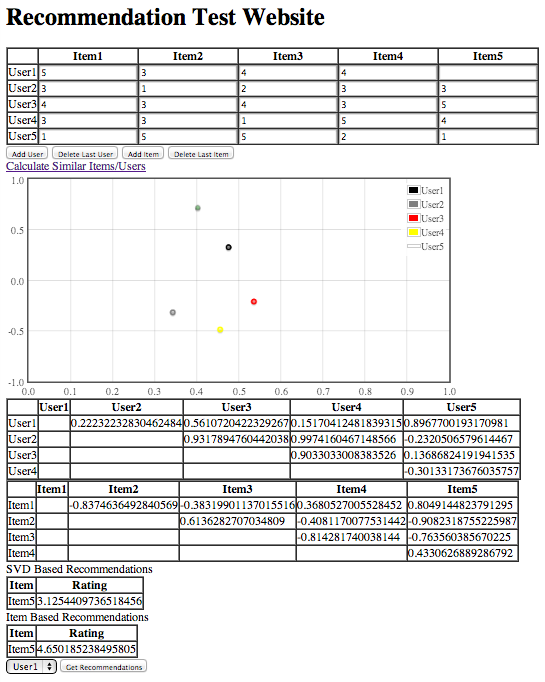
\includegraphics[width=\textwidth]{image/recommendationGui.png}
  \caption{The Graphical User Interface for The Recommendation Process}
  \label{pic:recommendationGui}
\end{figure}

The user interface is implemented with the \emph{backbone.js} library that provides models, collections and views for creating model view controller websites on the client side.
%dies wurde benoetigt, damit kein echter webservice mit file struktur usw gebaut werdem musste und kein weiteres framework benoetigt wurde
%es musste lediglich eine restful api erstellt werden sowie eine moeglichkeit um javascript dateien vom filesystem an den client zu schicken.
% backbone.js models expect restful api to work without configuration

\section{Architecture}
The system uses a service oriented architecture.
Thus the main components of the system namely the tagging process, the rating system and the different recommendation techniques are encapsulated in different services.
One advantage of that architectural choice is that the system can be spread on different servers.
This not just opens the possibility to run services that have high hardware requirements on different servers but also enables the choice to duplicate services.
The duplication of services can improve service downtimes and can decrease service respond times if the service is under high load.
A disadvantage of a service oriented architecture is that it is more complex to debug system errors because each service must be debugged on its own as well as the network communication between those services.
However one requirement for this system is that the single system components should be usable separately.
With a service oriented architecture each service can be used individually over a network communication.
The network communication protocol that is necessary for communicating with the services is the http protocol which is explained in subsection 3.1.3.
Figure ~\ref{serviceArchitecture} outlines the different services and the communication paths between those services.
%The http get and post request are the standard requests that are used by web
%browsers to send data.
%answer by http request respond
%explain http

\tikzstyle{decision} = [diamond, draw, fill=blue!20, 
    text width=4.5em, text badly centered, node distance=3cm, inner sep=0pt]
\tikzstyle{block} = [rectangle, draw, fill=blue!20, 
    text width=5em, text centered, rounded corners, minimum height=4em]
\tikzstyle{line} = [draw, -latex']
\tikzstyle{cloud} = [text width = 7.5em, text badly centered, draw, ellipse,fill=red!20, node distance=4cm,
    minimum height=2em]
    
\begin{figure}[h]
\begin{tikzpicture}[node distance = 2cm, auto]
    % Place nodes
    \node [cloud] (webservice) {Webservice};
    \node [cloud, right of=webservice] (recommendation) {Recommendation Service};
    \node [cloud, above right of=recommendation] (item) {Item-Based Recommendation Service};
    \node [cloud, below right of=recommendation] (svd) {SVD-Based Recommendation Service};
    \node [cloud, below of=recommendation] (tag) {Tagging Service};
    \node [cloud, below of=tag] (rating) {Rating Service};
    \node [cloud, right of=tag] (stw) {Query STW Service};
%   \node [block] (init) {initialize model};
%   \node [cloud, left of=init] (expert) {expert};
%   \node [cloud, right of=init] (system) {system};
%   \node [block, below of=init] (identify) {identify candidate models};
%   \node [block, below of=identify] (evaluate) {evaluate candidate models};
%   \node [block, left of=evaluate, node distance=3cm] (update) {update model};
%   \node [decision, below of=evaluate] (decide) {is best candidate better?};
%   \node [block, below of=decide, node distance=3cm] (stop) {stop};
    % Draw edges
%   \path [line] (init) -- (identify);
%   \path [line] (identify) -- (evaluate);
%   \path [line] (evaluate) -- (decide);
%   \path [line] (decide) -| node [near start] {yes} (update);
%   \path [line] (update) |- (identify);
%   \path [line] (decide) -- node {no}(stop);
%   \path [line,dashed] (expert) -- (init);
%   \path [line,dashed] (system) -- (init);
%   \path [line,dashed] (system) |- (evaluate);
    \path [line] (webservice) -- (recommendation);
    \path [line] (recommendation) |- (item);
    \path [line] (recommendation) |- (svd);
    \path [line] (webservice) |- (tag);
    \path [line] (webservice) |- (rating);
  \end{tikzpicture}
  \caption{The Service Architecture of the system}
  \label{serviceArchitecture}
\end{figure}


%Service oriented architecture why?
%communication diagram
%explain diagram
\section{Services}
The individual parts of the system are separated into different services this is illustrated in figure ~\ref{serviceArchitecture}.
Each service inherits from the HttpServer.
This HttpServer handles the decomposing of the http request, provides simple http routing and creates the http responses for the network communication.
Thus the services implement the service specific logic and provide methods for accessing this logic.
These methods are accessible for the router that is inherited by the HttpServer and provide a http path for each method in form of a string.
Consequently the services are accessible on their specific port with http post and http get requests that correspond to the http path.
These services return a standard http response that contains a json string as a return value.
%todo this section explains the different services that were developed for this thesis. Overall design pattern for the services \dots
%what is the service for 
%how to communicate with the service
\subsection{RecommendationService}
  %todo describe pipeline architecture
  The recommendation service controls the item based service and the svd based service.
  Therefore the single recommendation techniques can be regulated by editing the recommendation service. 
  This opens the possibility to use different recommendation approaches without much programming effort.
  \begin{center}
    \begin{tabular}{| l | l | l |}
       %&Low Scroll Time and Low Time Spend & Low Scroll Time and Medium Time Spend & Item3 & Item4 & Item5 \\ 
      \hline
      \multicolumn{3}{|c|}{RecommendationService } \\ 
      \hline \hline
      Standard Port & \multicolumn{1}{l}{13000} &\\ 
      \hline \hline
      Get Methods & Parameter: Type & Return Value\\ \hline
      /calculateSimilarities & - & \\ \hline
      \multirow{2}{*}{/calculateUserRecommendations} & user id: Integer & List (user, rating)\\
      & amount: Integer & \\ \hline
      \multirow{2}{*}{/calculateUserPrediction} & user id: Integer & List (user, rating)\\
      & item id: Integer &\\ %\hline
      %/calculateUserPredictionsItemBased & user id: Integer & \\ \hline
      %/calculateUserPredictionsSvdBased & user id: Integer & \\ 
      \hline \hline
      Post Methods & Parameter: Type & \\ \hline
      - & - & -\\ \hline
    \end{tabular} 
  \end{center}
  The \emph{/calculateSimilatities} method starts the item similarity calculation of the \emph{ItemBasedService} Service.
  After the calculation finishes the \emph{RecommendationService} Service starts the svd based similar user calculation of the \emph{SVDBasedService} Service.
  These similarity values are stored in the database by the individual service for future rating predictions.
  The \emph{/calculateUserRecommendations} method takes an user id, a number of predictions and a list of tags as parameters.
  This method forwards the parameters to the \emph{SVDBasedService} Service and returns the list of item rating pairs.
  The \emph{/calculateUserPredictions} method takes an user id and an item id as parameters.
  If the item id is empty the prediction for all items are calculated if enough similar item ratings exist.
  The final prediction calculation is handled by the \emph{SVDBasedService} Service. 



\subsection{ItemBasedService}
%der item based service ist verantwortlich fuer die item based recommendation berechnungen dh er berechnet die item similarities und kann 
  The \emph{ItemBasedService} is a service that is responsible for calculating the item similarities and to predict user ratings to decrease the sparsity of the user-item table.
  It is the implemented item based recommendation concept and therefore can be used as a part of the complete recommendation concept that is introduced in this thesis but it is a full functional recommendation system on its own.
  In the evaluation chapter section 4.3 the \emph{ItemBasedService} is used as a standalone recommendation system and the results are compared with the complete recommendation concept.
  \begin{center}
    \begin{tabular}{| l | l | l |}
       %&Low Scroll Time and Low Time Spend & Low Scroll Time and Medium Time Spend & Item3 & Item4 & Item5 \\ 
      \hline
      \multicolumn{3}{|c|}{ItemBasedService } \\ 
      \hline \hline
      Standard Port & \multicolumn{1}{l}{13100} &\\ 
      \hline \hline
      Get Methods & Parameter: Type & Return Value\\ \hline
      /calculateSimilarItems & - & - \\ \hline
      \multirow{2}{*}{/calculateUserPrediction} & user id: Integer & List (user, rating)\\
      & item id: Integer & \\ 
      \hline \hline
      Post Methods & Parameter: Type & \\ \hline
      - & - & -\\ \hline
    \end{tabular} 
  \end{center}

  The \emph{/calculateSimilarItems} method calculates the similarity between all items.
  The idea behind the similarity calculation is that the algorithm only considers to calculate the item similarity of items if they are rated together with other items by the same user.
  The algorithm ~\ref{alg:itemSim} is based on the work of \citet{amazon2003}.
  \begin{algorithm}
    \caption{Item Similarity Calculation}\label{alg:itemSim}
    \begin{algorithmic}[1]
      \Procedure{ItemSimilarity}{}
      \State items $\gets$ load all items
      \State seenTogether $\gets$ empty Set of item tupel
      \For{each $item_1$ in items}
        \State newItems $\gets$ empty Set of items
        \For{each user that rated $item_1$}
          \For{each $item_2$ that is rated by user}
            \If{$item_2 \neq item_1$ and seenTogether does not contain $(item_2, item_1)$} 
              \State add $(item_2, item_1)$ to seenTogether
              \State add $item_2$ to newItems
            \EndIf
          \EndFor
        \EndFor
        \State calculate similarities for $item_1$ and all items from newItems
      \EndFor

      \EndProcedure
    \end{algorithmic}
  \end{algorithm}
  Let N be the number of items in the system and M be the number of users who rated that item.
  Then as \citet{amazon2003} stated the worst case runtime of algorithm ~\ref{alg:itemSim} is $O(N^2M)$ but due to the reason that most rating tables are very sparse the runtime on a productive system is closer to $O(NM)$.
  The \emph{/calculateUserPrediction} method takes an user id and an item id as parameters.
  It calculates the rating prediction for the user-item pair and returns it as a list with one element.
  If the item id is empty it calculates the user predictions for all not rated items for the specific user and returns it as a list.
  %similarity calculation where too slow on own implementation for that reason a library is used.

\subsection{SVDBasedService}
  The \emph{SVDBasedService} implements the concept of the \emph{singular value decomposition} based recommendation system.
  This concept states that a user-item matrix can be decomposed into three matrices.
  Where the columns of one matrix responds to the user interest of the original user-item matrix.
  With these columns the similarity between the users is calculated and with the user similarities the recommendations are generated.
  The whole concept of the singular value decomposition based recommendation is explained in more detail in subsection 2.4.2.
  The \emph{SVDBasedService} service is responsible for calculating the recommendations after the item based service has decreased the sparsity of the rating table.
  However this service can be used as a stand alone recommendation system which is evaluated and compared with the complete recommendation system in section 4.3.

  \begin{center}
    \begin{tabular}{| l | l | l |}
       %&Low Scroll Time and Low Time Spend & Low Scroll Time and Medium Time Spend & Item3 & Item4 & Item5 \\ 
      \hline
      \multicolumn{3}{|c|}{SVDBasedService } \\ 
      \hline \hline
      Standard Port & \multicolumn{1}{l}{13200} &\\ 
      \hline \hline
      Get Methods & Parameter: Type & Return Value\\ \hline
      /calculateSimilarUsers & - & - \\ \hline
      \multirow{2}{*}{/calculateUserPrediction} & user id: Integer & List (user, rating)\\
      & item id: Integer & \\ 
      \hline \hline
      Post Methods & Parameter: Type & \\ \hline
      - & - & -\\ \hline
    \end{tabular} 
  \end{center}

  The \emph{/calculateSimilarUsers} method executes the calculation of the similar user values.
  This process is split into four steps.
  At first the user-item matrix is created out of the rating table.
  After that the method calculates the singular value decomposition of the matrix.
  For this task the \emph{Apache commons-math} library is used.
  This library is a general math library with strong linear algebra algorithms developed and maintained by \emph{The Apache Software Foundation}.
  %todo why am i using this library
  The third step is the approximation of the U matrix that is one of the resulting matrices from the singular value decomposition.
  Finally the similar users are generated by calculating the cosine similarity between all columns of the U matrix.
  This method does not have a return value. 
  All similar user values are stored in the database for future calculations.
  The \emph{/calculateUserPrediction} method calculates a prediction for the specified user-item pair.
  If no item is specified the method calculates a prediction for all items that are not rated by the specified user.
  For this process the system generates a list of the most similar users $U_{sim}$.
  With these similar users it generates a list of items that these users rated but are unknown to the current user.
  For each item that is in the unknown item list the system calculates the prediction for the user-item pair as described in subsection 2.4.2.
  These predictions are returned as a list of user-item tupel.


\subsection{TaggerService}
  The \emph{TaggerService} is the implementation of the tagging concept.
  This concept describes the process of finding the right tags for a text.
  For this process the system creates a deterministic levenshtein automata for each word in a text.
  Every one of these deterministic levenshtein automatas reads the complete \emph{STW Standard Thesaurus Economics} if a word from the \emph{STW} ends in a final state the word is used as a tag for the text.
  More details about the tagging concept can be found in section 2.3.
  \begin{center}
    \begin{tabular}{| l | l | l |}
       %&Low Scroll Time and Low Time Spend & Low Scroll Time and Medium Time Spend & Item3 & Item4 & Item5 \\ 
      \hline
      \multicolumn{3}{|c|}{TaggingService } \\ 
      \hline \hline
      Standard Port & \multicolumn{1}{l}{11000} &\\ 
      \hline \hline
      Get Methods & Parameter: Type & Return Value\\ \hline
      - & - & - \\ 
      \hline \hline
      Post Methods & Parameter: Type & \\ \hline
      /tagText & text: String & list of tags\\ \hline
    \end{tabular} 
  \end{center}
  The \emph{tegText} method takes a text as parameter. 
  The single words of the text are extracted into a list.
  For each word in this list a deterministic levenshtein automata is generated.
  For this process the service creates a finite automata for each word with a specific degree.
  A degree states the maximum allowed levenshtein distance between the word for which the automata is generated and the word that the automata can read.
  This degree depends on the word size.
  For a word with more than five letters a degree of three is used otherwise a degree of one is used.%todo this has to match the concept
  %\todo{Add Algorithm here}
  The states are written as tupel of the form (c, d) where c denotes the current position in the word and d denotes the current levenshtein distance between the prefix of the original word and the word that the automata reads.
  For each letter in a word W with a length of n four transitions are created if the levenshtein distance of the current state is smaller than n.
  These four transitions represent reading a correct letter, deleting a letter, inserting a letter and substituting a letter.
  The last states that are reached thru the last letter do not get any transitions by this process.
  Consequently the next step is to insert the missing \emph{insertion} transitions for these last states where the current position in the word is the size of the word.
  These insertions are needed because the word that is read might be longer than the original word and therefore letters must be added to the original word up to the maximum degree.
  The last step for creating this finite automata is to mark all of the last states where the current position in the word is the size of the word as final states.
  This finite levenshtein automata is transformed into a deterministic finite levenshtein automata.
  \todo{add transformation algorithm}


\subsection{RatingService}
%load javascript add user id item id to the page as js
%if item is unknown return javascript that reads the question and returns it to the rating service this service sends it to the tagging service
%with the tagging information it creates a new item
  \begin{center}
    \begin{tabular}{| l | l | l |}
      \hline
      \multicolumn{3}{|c|}{RatingService } \\ 
      \hline \hline
      Standard Port & \multicolumn{1}{l}{12000} &\\ 
      \hline \hline
      Get Methods & Parameter: Type & Return Value\\ \hline
      - & - & - \\ 
      \hline \hline
      Post Methods & Parameter: Type & Return Value\\ \hline
      \multirow{4}{*}{/rateItem} & user id: Integer & JavaScript if item is unknown\\
      & item id: Integer &  \\
      & time spend: decimal &  \\
      & time scroll: decimal &  \\ \hline
    \end{tabular} 
  \end{center}

\subsection{WebService}

\chapter{Evaluation}
This chapter is about \dots
\section{Rating}
The evaluation for the rating system refers to the rating concept from subsection 2.2.5.
This concept is build upon the researches from \citet{claypool2001} who evaluated different user interactions and compared those with explicit user ratings.
The two user interactions that performed the best with an accuracy of about 70\% to the user ratings are the time a user spend on a website and the time a user scrolls.
Each of the measured times of the user interactions are split into segments depending on the truncated mean time of all user times.
Yielding a scale that enables the system to calculate ratings based on the user interactions.
Based on this scale the ratings are calculated separately and are combined to the total rating by calculating the average of both ratings.
This total rating is evaluated with the research data from \citet{claypool2001} in this section.
For the rating evaluation an item test website is created.
This test website is a standard html website with a high of 2000px.
Consequently there is the possibility to scroll on a standard screen resolution.
Additionally the item test website has a truncated mean time for the time a user spends on the website and another truncated mean time for the time a user scrolls on the website.
For these truncated mean times the average times from the users of the field test from \citet{claypool2001} that rated websites with a 3 are used.
These average times are 5.267 seconds for the time a user scrolls and 21.217 seconds for the time a user spends on a website.
Finally users who visits the website are simulated.
Those users are interacting with the website according to the times of \citet{claypool2001} field experiment.
Therefore the ratings that the simulated users generate can be compared to the data from the team of \citet{claypool2001}.
\begin{displaymath}
  \begin{tabular}{c c c c c c}
     %&Low Scroll Time and Low Time Spend & Low Scroll Time and Medium Time Spend & Item3 & Item4 & Item5 \\ 
     Scroll Time & 5 & 3 & 4 & 4 &  \\  
     Scroll Time Rating \\
    Time Spend & 3 & 1 & 2 & 3 & 3\\ 
    Time Spend Rating \\
    Total Rating & 1 & 5 & 5 & 2 & 1\\ 
  \end{tabular} 
\end{displaymath}

% The single ratings match with the ratings of \citet{claypool2001}.
% The total ratings reflect the expected ratings.
% However the total rating is derived from the data of \citet{claypool2001} and it would have been desirable to conduct a field experiment but unfortunately due to the lack of time this was not possible.


%%daher wurde getestet ob unterschiedliche surfverhalten unterschiedliche ratings hervorbringen. und ob diese mit den in chapter 2 section 2.2 subsubsection 2.2.5 vorgestellten theorien uebereinstimmen
%%versuchsaufbau fuer die evaluation wurde eine test webseite erstellt diese hat eine truncated mean time erhalten die aus den aussagen von claypool et al hervorgingen.
%anschliessend wurden seiten aufrufe simuliert die mit den werten von claypool uebereinstimmten und ueberprueft ob die ergebnisse wiederspiegeln was man erwartet.
\section{Tagging}
This section evaluates the tagging process that was introduced in subsection 2.3.2.
The concept behind the tagging process is to create a \emph{levenshtein automata} for every word in an item\footnote{An item represents a question and answer} and read each word from the \emph{STW Standard Thesaurus Economics} into the automata.
If the word ends in a final state it is used as a tag for the item.
Such a \emph{levenshtein automata} is a deterministic finite automata that can decide in linear time if a word has a \emph{levenshtein distance} smaller than a desired $n\in\mathbb{N}$.
Four different texts are created for the evaluation process. 
At each of these four texts are 30\% of the words from the \emph{STW Standard Thesaurus Economics}.
However, not all of the words are in the same form as they are found in the \emph{STW Standard Thesaurus Economics}.
Thus the tagging algorithm has to match the words from the item with the correct words from the STW.
After each test the matched words are compared to the words that should have matched.
Moreover, the time that the algorithm needed is evaluated.

\begin{displaymath}
  \begin{tabular}{c c c c c c}
     &STW Words & Words Matched & Wall Clock Time \\ 
     10 Words & 3 & 3 & 4 \\  
     100 Words & 30 & 28 & 10\\
    500 Words & 150 & 145 & 30 \\ 
    1000 Words & 300 & 280 & 100 \\
  \end{tabular} 
\end{displaymath}

%erstelle text mit keywords die im STW enthalten sind und daher gefunden werden muessen. stelle fest das die meisten gefunden werden aber wenn woerter zu stark veraendert werden nicht mehr gematcht werden was zu erwarten war
%test 10 words 100 words 500 words 1000 words with the service
%compare original levenshtein to new levenshtein
\section{Recommendation}
This section evaluates the different recommendation approaches that are explained in subsection 2.4.4.
These different approaches are the item-based recommendation, the svd-based recommendation, the item-based recommendation that uses the V matrix from the svd and the hybrid approach that uses item-based predictions to decrease the sparsity of the rating table and the svd-based approach for recommendations.\todo{improve this}
The evaluation process of the recommendation system is split into two parts.
At first the performance of the different approaches is evaluated by using the wall clock time.
Second the accuracy of the different concepts is compared.
For this task the \emph{MovieLens} database is used.
The \emph{MovieLens} database includes 100.000 ratings from 943 users for 1682 movies.
These ratings were collected by the \emph{GroupLens} research project from the University of Minnesota.
To compare the accuracy of the recommendation systems the \emph{Mean Absolute Error} (MAE) is used.
This metric is according to \citet{sarwar2001} most commonly used for evaluating recommendation systems.
The MAE is a statistical metric that compares the calculated user-item ratings from the recommendation system with real user-item ratings. 
For this process the recommendation system is trained with for example 80\% of a test rating database and afterwards the remaining 20\% are used to check if the recommendations are correct. 
\begin{definition}[Mean Absolute Error]
  Let $p_{i, j}$ be the predicted rating for user i and item j and let $q_{i, j}$ be the real rating for user i and item j.
  Then the following formula calculates the MAE.
  MAE = 
\end{definition}

\subsection{Performance of the Recommendations}
The following table displays the different recommendation approaches together with the wall clock time.
Therefore \dots
The hybrid approach is the slowest of all recommendation processes this was expected because it uses two recommendation processes after another.
\subsection{Accuracy of the Recommendations}
As mentioned above the accuracy of the recommendations is measured with the \emph{Mean Absolute Error}.
The following table outlines the results from the different recommendation system approaches.



%Evaluating Collaborative Filtering Recommender Systems
%JONATHAN L. HERLOCKER
% Finally, there is a significant challenge in deciding what combination of mea- sures to use in comparative evaluation. We have noticed a trend recently�many researchers find that their newest algorithms yield a mean absolute error of 0.73 (on a five-point rating scale) on movie rating datasets. Though the new al- gorithms often appear to do better than the older algorithms they are compared to, we find that when each algorithm is tuned to its optimum, they all produce similar measures of quality. We�and others�have speculated that we may be reaching some �magic barrier� where natural variability may prevent us from getting much more accurate. In support of this, Hill et al. [1995] have shown
% ACM Transactions on Information Systems, Vol. 22, No. 1, January 2004.
% Evaluating Collaborative Filtering Recommender Systems � 7
% that users provide inconsistent ratings when asked to rate the same movie at different times. They suggest that an algorithm cannot be more accurate than the variance in a user�s ratings for the same item.


% \subsubsection{Item-Based}
% \subsubsection{Singular Value Decomposition}
% \subsubsection{Hybrid Of Item-Based and Singular Value Decomposition}
\chapter{Future Work}
\section{Rating System}
\section{Tagging Service}
Direct implementation of the deterministic levenshtein automata, table based approach.
Save levenshtein automatas from all \emph{STW Standard Thesaurus Economic} words with an appropriate datastructure.
\section{Recommendation System}

\appendix

%%%%%%%%%%%%%%%%%%%%%%%%%%%%%%%%%%%%%%%%%%%%%%%%%%%%%%%%%%%%%%%%%%
%%                                                              %%
%%                     Literaturverzeichnis                     %%
%%                                                              %%
%%%%%%%%%%%%%%%%%%%%%%%%%%%%%%%%%%%%%%%%%%%%%%%%%%%%%%%%%%%%%%%%%%

\bibliography{bib}       %% statt mybib Name der eigenen .bib-Datei einsetzen 
\bibliographystyle{plainnat}

\end{document}
